%%% PREAMBLE 
\documentclass[sn-vancouver]{sn-jnl}

\usepackage{bm}
%\usepackage{caption}
\usepackage{float}
%\usepackage{listings}
\usepackage{multirow}
\usepackage{siunitx}
%\usepackage{subcaption}
%\usepackage{soul}
%\usepackage{adjustbox}
\usepackage{hyperref}
%\usepackage{academicons}
\usepackage[numbers]{natbib}

\graphicspath{ {./Figures/} }

%\setlength{\marginparwidth}{2cm}


\begin{document}
%%%%%%%%%%%%%%%%%%%%%%%%%%%%%%%%%%%%%%%%%%%%%%%%%%%%%%%%%%%%
%%% ARTICLE SETUP
%%%%%%%%%%%%%%%%%%%%%%%%%%%%%%%%%%%%%%%%%%%%%%%%%%%%%%%%%%%%
\title[Identifying signatures of proteolytic stability and monomeric propensity ]{Identifying signatures of proteolytic stability and monomeric propensity in \emph{O}-glycosylated insulin using molecular simulation}

\author[1]{Wei-Tse Hsu} % ORCID: 0000-0001-6167-5480
\author[2]{Dominique A. Ramirez} % ORCID: 0000-0002-2944-8250
\author[3]{Tarek Sammakia} % ORCID: 0000-0003-3703-5672
\author*[4]{Zhongping Tan}\email{zhongping.tan@imm.pumc.edu.cn}  % ORCID: 0000-0002-9302-150X
\author*[1]{Michael R. Shirts}\email{michael.shirts@colorado.edu} % ORCID: 0000-0003-3249-1097

\affil[1]{Department of Chemical \& Biological Engineering, University of Colorado Boulder, Boulder, CO, USA 80309}
\affil[2]{Department of Biochemistry, University of Colorado Boulder, Boulder, CO, USA 80309}
\affil[3]{Department of Chemistry, University of Colorado Boulder, Boulder, CO, USA 80309}
\affil[4]{Institute of Materia Medica, Chinese Academy of Medical Sciences, Peking Union Medical College, Beijing, 100050, China}

%\corr{michael.shirts@colorado.edu}{MRS}
%\corr{zhongping.tan@imm.pumc.edu.cn}{ZT}


%%%%%%%%%%%%%%%%%%%%%%%%%%%%%%%%%%%%%%%%%%%%%%%%%%%%%%%%%%%%
%%% ARTICLE START
%%%%%%%%%%%%%%%%%%%%%%%%%%%%%%%%%%%%%%%%%%%%%%%%%%%%%%%%%%%%

%\begin{document}
 
%\maketitle

\abstract{Insulin has been commonly adopted as a peptide drug to treat diabetes given its ability to facilitate the uptake of glucose from the blood. The development of oral insulin remains elusive over decades owing to its susceptibility to the enzymes in the gastrointestinal tract and poor permeability through the intestinal epithelium upon dimerization. Recent experimental studies have revealed that certain \emph{O}-linked glycosylation patterns could enhance insulin's proteolytic stability and reduce its dimerization propensity, but the understanding of such phenomena at the molecular level is still evasive. To address this challenge, we proposed and tested several structural determinants that could potentially influence insulin's proteolytic stability and dimerization propensity. We used these as the metrics to assess the properties of interest from 10 $\mu$s aggregate molecular dynamics of each of 12 targeted insulin glyco-variants from multiple wild-type crystal structures. We found that glycan-involved hydrogen bonds and glycan-dimer occlusion were useful metrics predicting the proteolytic stability and dimerization propensity of insulin, respectively, as was in part the solvent-accessible surface area of proteolytic sites, while other plausible metrics were not generally predictive. This work helps better explain how \emph{O}-linked glycosylation influences the proteolytic stability and monomeric propensity of insulin, illuminating a path towards rational molecular design of insulin glycoforms.}

\keywords{insulin, \emph{O}-glycosylation, stability, protein degradation, molecular dynamics}


\maketitle

%===============================
% Introduction
%===============================
\section{Introduction}
Insulin has been widely used as a peptide drug to treat both type 1 and type 2 diabetes mellitus by promoting the absorption of glucose from the blood into the liver, fat, and skeletal muscle cells. While it is usually administered via subcutaneous injections, excessive injections could lead to non-compliance by patients owing to injection pain and associated side effects, including trypanophobia, lipodystrophy, and peripheral hyperinsulinemia~\cite{carino1999oral}. As such, there has been a growing interest in the development of an insulin drug for oral administration~\cite{carino1999oral, fonte2013oral, gedawy2018oral}. Orally ingested insulin not only avoids the aforementioned side effects of subcutaneous administration, but also has the advantage of reaching the liver at high concentration via the portal vein before reaching systemic circulation, which better mimics the physiology of endogenous secretion by the pancreas and provides a better glucose homeostasis~\cite{hoffman1997pharmacokinetic, owens2002new}. 
However, developing oral insulin remains a major challenge because of its susceptibility to proteases in the digestive system of the human body and poor permeability across the intestinal epithelium upon dimerization, which leads to overall low absorption efficiency~\cite{bruno2013basics}. Therefore, proteolytic stability and dimerization propensity are two of the most important controlling factors when developing oral insulin drugs. During past years, a wide array of strategies, including chemical modifications~\cite{hinds2002effects, clement2002oral}, nano-particulate carrier systems~\cite{deng2017selenium, bhattacharyya2017preparation, zhou2020nanocomposite}, and utilization of protease inhibitors~\cite{agarwal2000oral}, have been shown to have varying degrees of success in improving these two insulin properties. 

Glycosylation is one of these chemical modifications strategies and has shown significant promise in enhancing the proteolytic stability and monomeric propensity of various kinds of proteins~\cite{kayser2011glycosylation, raju2006glycosylation,russell2009site}. While \emph{N}-linked glycosylation has been more studied~\cite{losev2019novel,van2004role, sareneva1995n} due to better controllability and the ease of chemical synthesis, \emph{O}-linked glycosylation has a larger diversity of carbohydrate structures and potentially a greater ability for tuning biophysical properties of glycoproteins. Guan et al. systematically investigated different glycosylation patterns, including glycosylation sites, glycan sizes, and glycan structures~\cite{guan2018chemically}. Their study suggested the superiority of \emph{O}-mannosylation of insulin B-chain Thr27 to other studied glycosylation patterns in increasing the proteolytic stability against $\alpha$-chymotrypsin and decreasing the dimerization propensity of insulin, while still maintaining full biological activity. However, there is a lack of quantitative understanding of how insulin properties are influenced by the interactions between the attached sugar molecules and insulin residues, particularly at the molecular level. 

Recent advances in molecular simulation methods and greater availability of computing resources allow much more comprehensive exploration of biomolecular systems at the atomistic level than was previously possible. A number of previous studies have shown molecular dynamics (MD) simulations to be a powerful tool for understanding the properties and dynamics of insulin. Mark et al.~\cite{mark1991conformational} and Zoete et al.~\cite{zoete2004comparison} found that the insulin monomer is more flexible than the dimer. Zoete et al.~\cite{zoete2004comparison} additionally confirmed the high flexibility in the B-chain C-terminus of insulin, which was consistent with the experimental data. Later, Yang~\cite{yang2011pegylation} et al. used simulated annealing~\cite{pincus1970letter} to probe how PEGylation enhanced the stability and potency of insulin, discovering that an optimal chain length existed for PEGglyated insulin pharmaceuticals. More recently, with steered molecular dynamics~\cite{isralewitz2001steered} and replica-exchange umbrella sampling~\cite{sugita2000multidimensional}, Antoszewski et al.~\cite{antoszewski2020insulin} revealed different pathways of insulin dimer dissociation and characterized relevant energetic and structural features of the process. Busto-Moner et al. ~\cite{busto2021structural} presented a pipeline integrating parallel tempering ~\cite{hansmann1997parallel, earl2005parallel}, the integrated variational approach for conformational dynamics (IVAC) ~\cite{nuske2014variational, lorpaiboon2020integrated}, Markov state model (MSM) ~\cite{prinz2011markov, bowman2013introduction}, and Perron cluster analysis (PCCA) ~\cite{schutte1999direct} for sampling the wild-type insulin ensemble and they concluded three important elements of disorder common in the insulin ensemble at a low pH value.

In this study, we aim to identify structural determinants from MD simulations of glycosylated insulin that lead to enhanced proteolytic stability against $\alpha$-chymotrypsin or reduced dimerization propensity. Specifically, we performed molecular dynamics simulations for each of the 12 insulin glycoforms (GFs) (Figure \ref{sys_of_interest}) studied in the experimental work~\cite{guan2018chemically} done by Guan et al. Each of the glycoforms was built upon five different wild-type models resolved by different methods/groups to encapsulate a wider variety of initial configurations so as to sample the conformational ensemble more comprehensively. Based on the proteolytic degradation mechanism by $\alpha$-chymotrypsin~\cite{schilling1991degradation} and the structural characteristics of insulin, we proposed several potential metrics for assessing the two insulin properties, including solvent-accessible surface area (SASA), secondary structures, the existence of glycan-involved hydrogen bonds, and the occlusion between the glycan and the dimer interface. A previous study~\cite{chaffey2017structural} found that greater conformational rigidity of a carbohydrate binding module (CBM) protein was associated with larger proteolytic stability of glycoforms, thus disfavoring reaction-capable transition states. However, the overall conformational rigidity of insulin is significantly different from CBM, and thus more specific measures of transition state accessibility were used, such as the $\beta$-sheet propensity, which more specifically takes the structural features of the known $\alpha$-chymotrypsin transition state into account.
\begin{figure}[H]
\centering
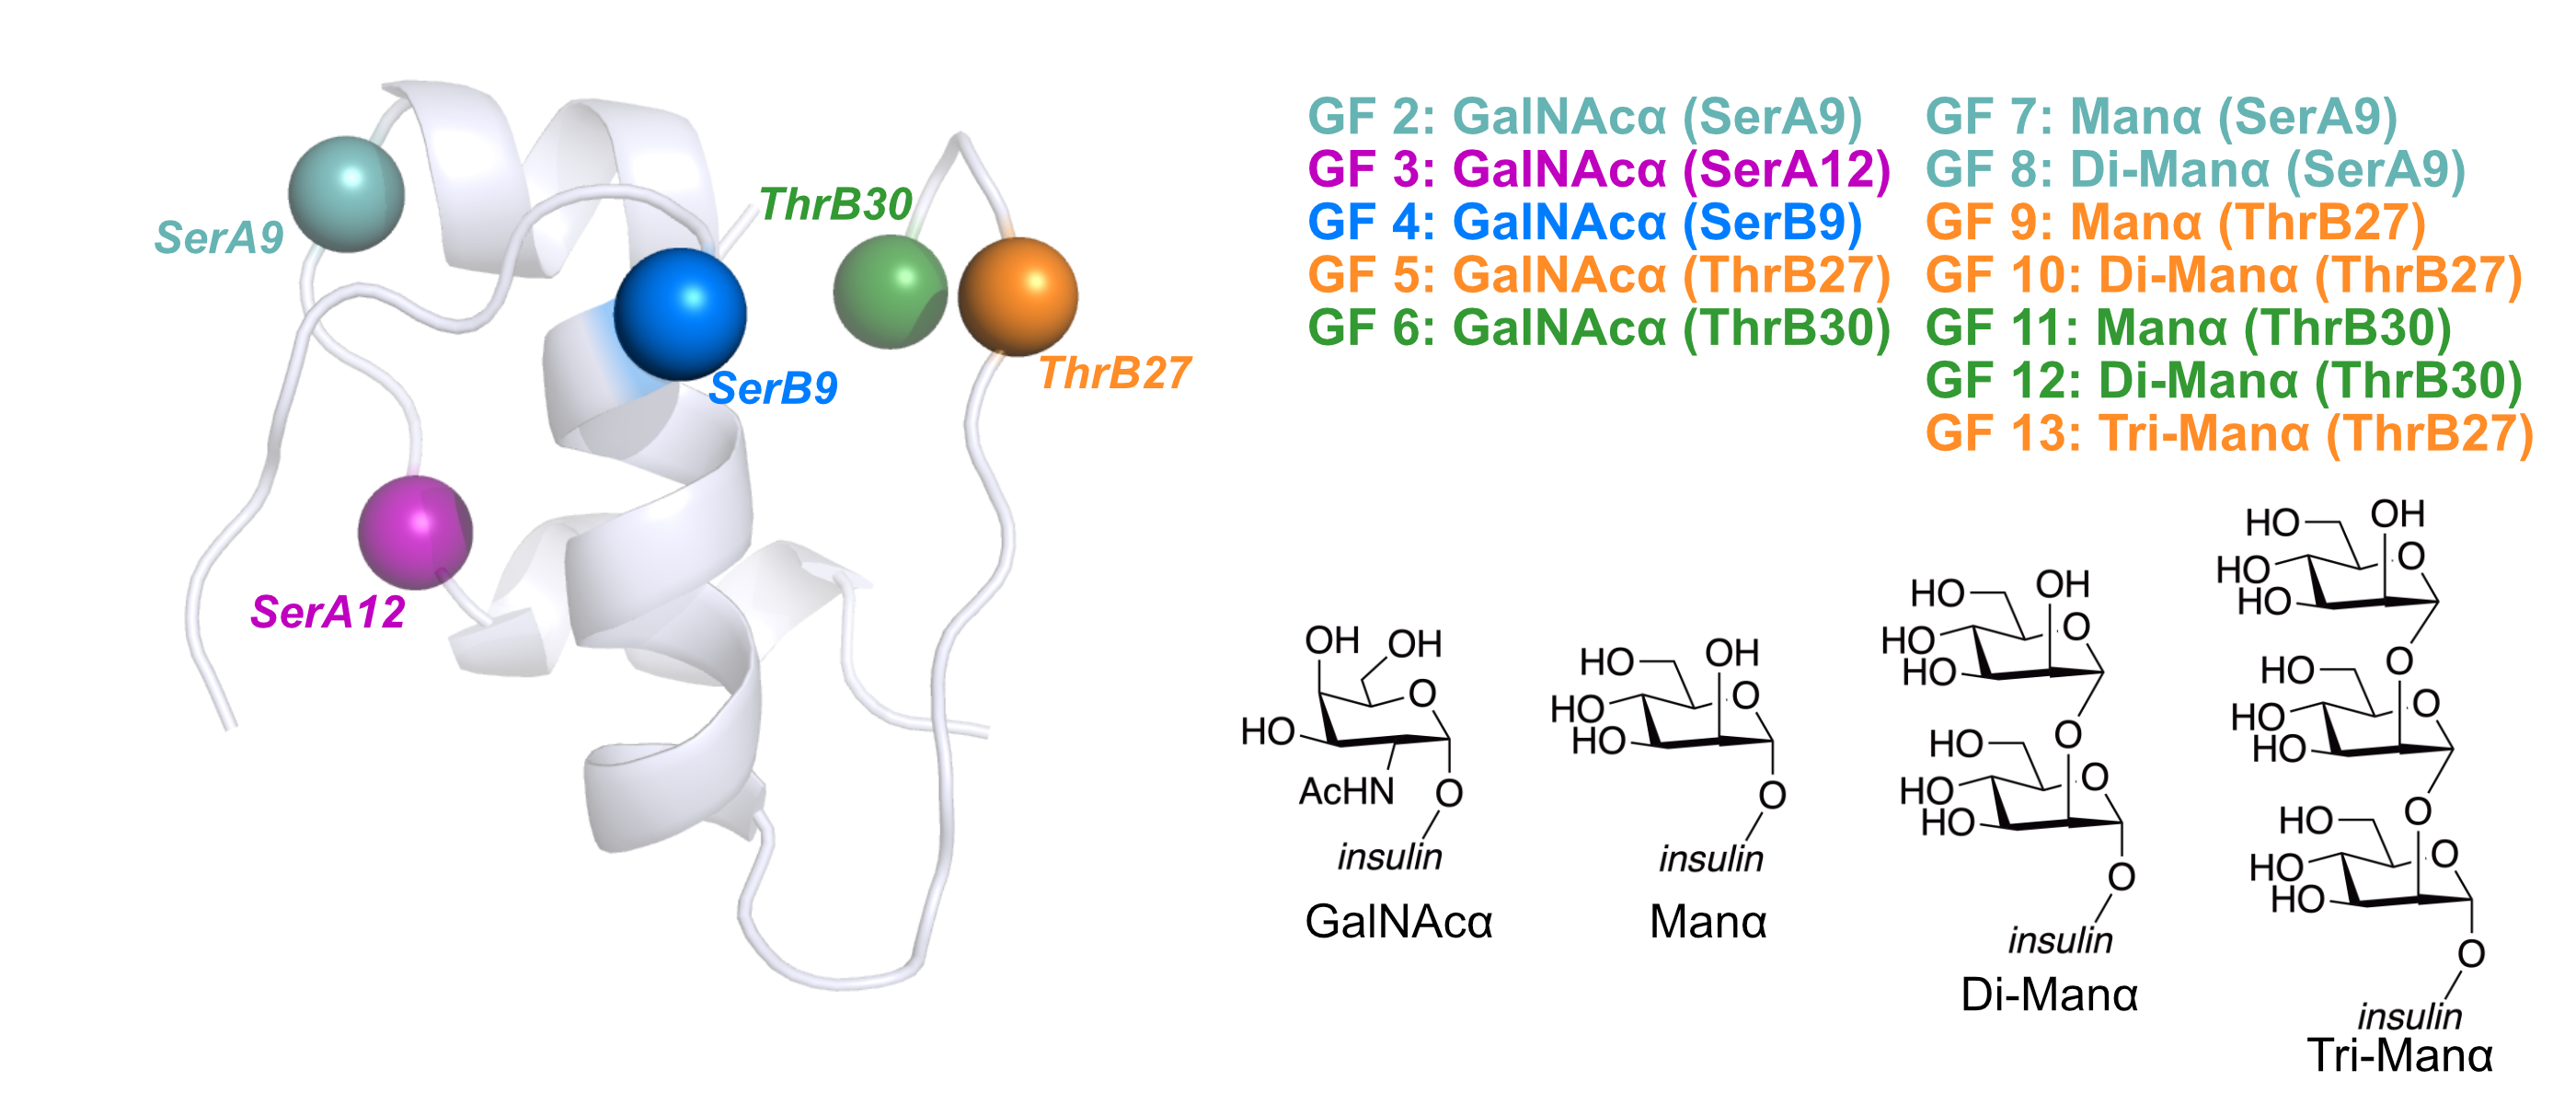
\includegraphics[width=\textwidth]{Figures/Fig_glycan_positions.png}
\caption{Structures of a human insulin monomer and glycoforms studied in this work. Two kinds of sugar moieties (\emph{N}-acetylgalactosamine (GalNAc) and mannose (Man) in the $\alpha$-anomer) with varying lengths (e.g. a mannose monomer, dimer, or trimer) were attached to five different glycosylation sites of insulin, including SerA9 (teal), SerA12 (purple), SerB9 (blue), ThrB27 (orange) and ThrB30 (green) all represented as beads. The glycosylation pattern of each glycoform is implied by its name---for example, GalNAc$\alpha$ (SerA9) represents the glycoform having an \emph{N}-acetylgalactosamine (GalNAc) attached to the A chain Ser9 residue. Note that for glycoforms having a mannose dimer or trimer as the glycan, the linkages between monomers were all $\alpha$-1,2-linkages, so Tri-Man$\alpha$ (ThrB27) refers to the glycoform containing an $\alpha$-1,2-linked tri-mannose at the B chain Thr27 residue.}
\label{sys_of_interest}
\end{figure}
Notably, both the proteolytic stability and dimerization propensity are related to transformation processes that require overcoming free energy barriers. The proteolytic stability can be directly associated with the free energy barrier of the formation of the conformational ensemble corresponding to the transition state in the proteolytic degradation by $\alpha$-chymotrypsin. Similarly, dimerization propensity is strongly correlated with the free energy barrier to dimerization. While these free energy differences could serve as more direct measures for the two biophysical properties of interest, calculations of such free energy differences are far from trivial. The reason lies in the fact that the timescale of the binding/unbinding events between an insulin monomer and an $\alpha$-chymotrypsin or between two insulin monomers are prohibitively long. This necessitates the use of advanced sampling techniques to accelerate the sampling of the configurational space of the system of interest, such as umbrella sampling~\cite{torrie1977nonphysical} or alchemical transformations~\cite{sugita2000replica, lyubartsev1992new}. However, such free energy methods are usually much more complicated and computationally expensive than standard MD simulations of the same length. The increase in the system size of insulin/protease complex or insulin dimer calculations adopting either method could easily increase the computational cost significantly beyond the scope of what is possible to screen large numbers of insulin modifications.  Advanced configurational sampling approaches can often be significantly difficult to set up and interpret, thus making easy screening impossible.

Therefore, instead of considering simulations of an insulin-$\alpha$-chymotrypsin complex and an insulin dimer, we worked to develop metrics for proteolytic stability and dimerization propensity based on standard MD simulations of monomers and their glycosylated analogs. The hypothesis is that the insulin monomer that participates in either a complex with $\alpha$-chymotrypsin or an insulin dimer should encode at least some important structural insights into both the proteolytic stability and the dimerization propensity. As long as we are able to explore the configurational space of monomer-based structures sufficiently, the conformational ensembles we get from the simulations should shed light on developing reasonable metrics for the two insulin properties. 

Given the output MD trajectories, all metrics were measured for each glycoform structure. They were later compared with the experimental work for assessing the efficacy. Notably, we found that at minimum 5 $\times$ 2000 ns = 10 $\mu$s of simulation was necessary to capture the structural characteristics of the insulin ensembles. This aggregate length is, to our knowledge, one of the longest among all the computational studies of human insulin. In addition, our study is not only one of the very few studies that characterize conformations of insulin with a covalently attached moiety, but is also unique as the first study that correlates molecular dynamics simulations to the proteolytic stability of these proteins. Our investigation facilitates a better understanding of the underlying mechanism of how different \emph{O}-glycosylation patterns influence insulin properties, which could be useful in guiding the design of insulin glyco-variants with better properties for oral delivery.

% %===============================
% % Methodology
% %===============================
\section{Methodology}
\subsection{Molecular dynamics simulations}
To reduce sampling bias of our MD simulations and ensure that our analysis results were not dependent on the initial configuration of insulin, in our study, we built each of the 12 glycoforms on 5 wild-type (WT) structures resolved by different groups using different methods, whose PDB IDs were 4EYD, 4EY9, 4EY1, 3I3Z, and 2MVC, respectively (Figure \ref{starting_structures}A). These initial models were chosen based on whether they were resolved in a complex or as a monomer. For example, 4EYD, 4EY9, and 4EY1 were all crystallized in complex with Zn$^{2+}$ as a hexamer composed of a dimer in 3-fold symmetry~\cite{favero2013structural}. They represented high-resolution human insulin structures from pharmaceutical formulations. 3I3Z and 2MVC, on the other hand, were representative of monomeric insulin structures. 3I3Z was resolved by X-ray crystallography under low gravity conditions so that the asymmetric unit of insulin was a monomer~\cite{timofeev2010x}. 2MVC was resolved by NMR spectroscopy under acidic conditions, which is known to favor the monomeric form of insulin~\cite{kvrivzkova2014structural}.

For those models resolved in the dimeric form, including 4EYD, 4EY9, and 4EY1, we extracted the insulin monomer from the dimer conformation. For 3I3Z, which was resolved as a monomer with the last residue on the B-chain mutated into an alanine, we used PyMOL~\cite{delano2002pymol} to mutate the residue back to a threonine to match the standard sequence of human insulin. Lastly, for the NMR-resolved 2MVC, we simply took the first model from the PDB file of the resolved ensemble. Notably, even if monomers extracted from a dimer conformation could potentially suffer from biases from experimental conditions that favor dimer resolution, as later shown, these biases did not have noticeable influences on the consistency of our methods. 

\begin{figure}[H]
\centering
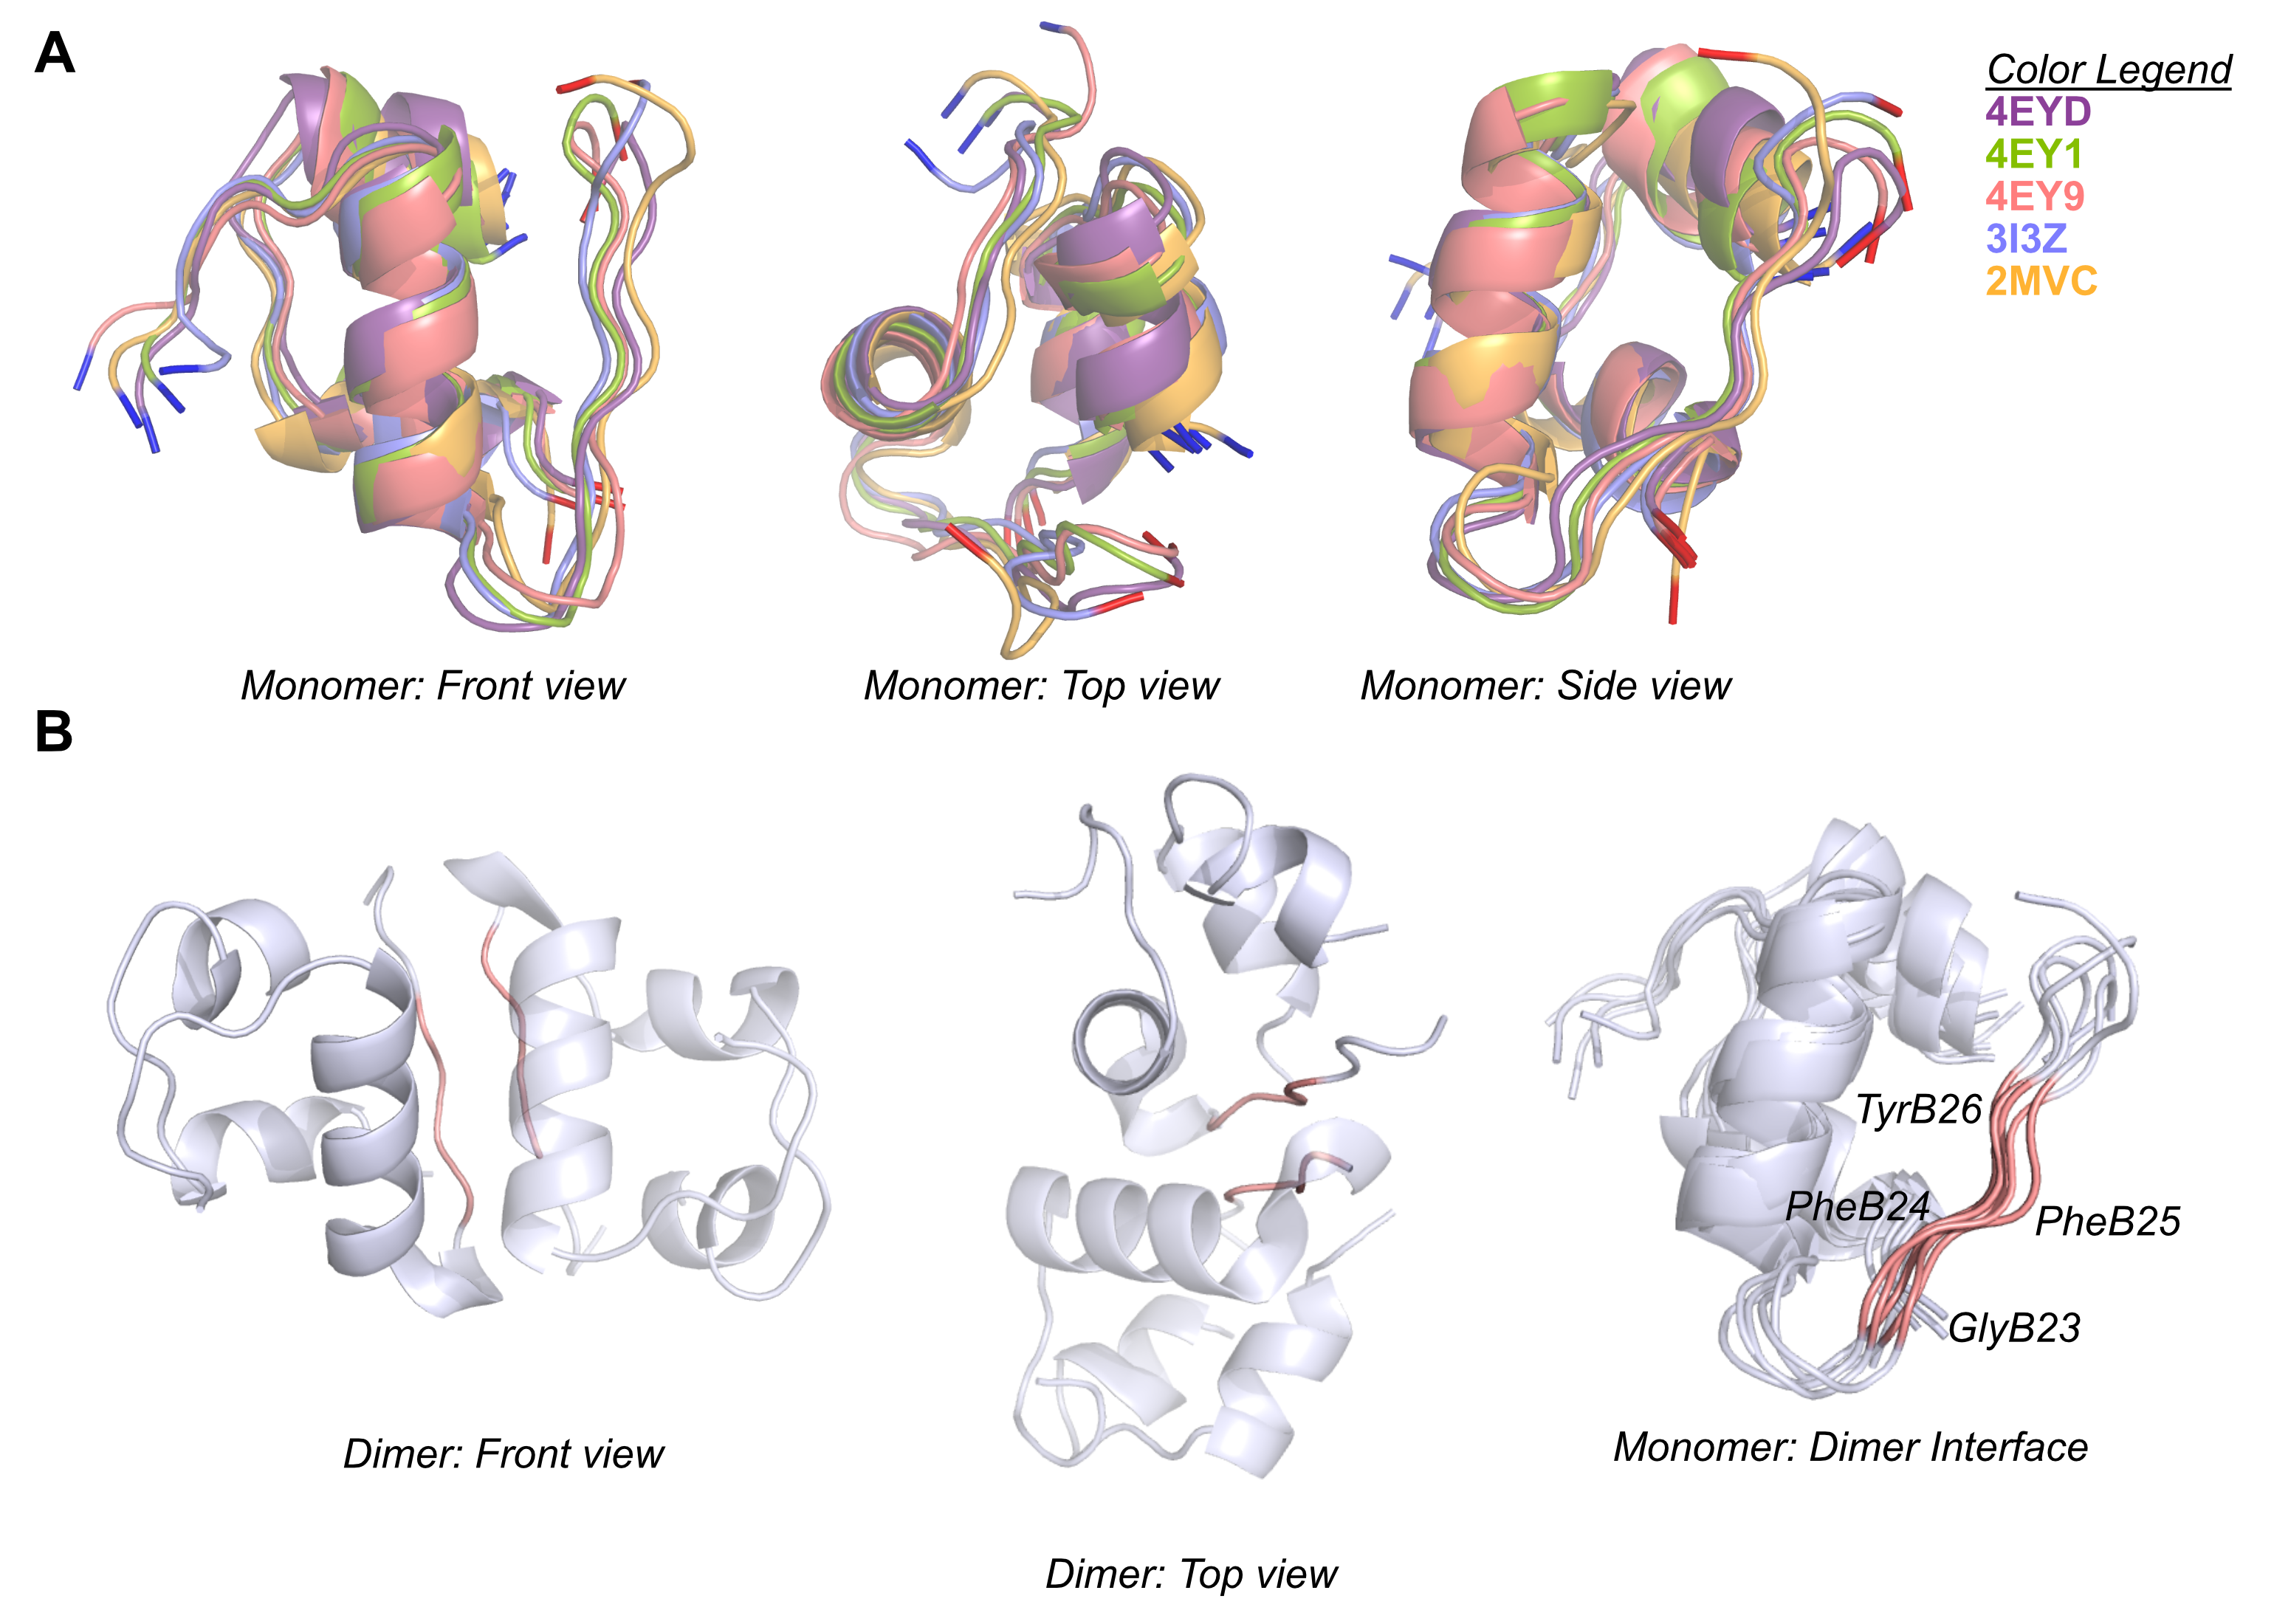
\includegraphics[width=\textwidth]{Figures/Fig_WTmodels_dimerInterface.png}
\caption{Structures of wild-type insulin models used in this study. (A) The initial monomer structures, after equilibration and before production simulation, are superimposed and are shown from different views. (B) Representative dimer structure illustrating the dimerization interface. The 3I3Z crystal structure was used to reconstruct an insulin dimer in the first two images. Residues GlyB23--TyrB26 (salmon) are highlighted. The last image shows the superimposed equilibrated wild-type structures with residue labels for the dimer interface.}
\label{starting_structures}
\end{figure}

After extracting the monomer structure from each of the initial models, we used the H++ server (version 3.2)~\cite{anandakrishnan2012h++, myers2006simple, gordon2005h++}, which also parameterized the protein with the AMBER ff14SB force field, to assign reasonable protonation states corresponding to the pH values adopted in experiments. Specifically, in the work~\cite{guan2018chemically} by Guan et al., the experiments of $\alpha$-chymotrypsin digestion (for estimating the $\alpha$-chymotrypsin half-life, hence the proteolytic stability) and analytical ultracentrifugation (for estimating the monomer/dimer population, hence the dimerization propensity) were conducted at pH 8.0 and pH 7.4, respectively. These two pH values respectively correspond to the typical pH values in the pancreatic tract (pH 7.5 to pH 8.0 ~\cite{mcqueen2017comprehensive}) and small intestine (pH 6 to pH 7.4~\cite{fallingborg1999intraluminal}) of human body. Around these pH values, the total charges of insulin were predicted to be -1 or -2,  depending on the pK$_{1/2}$ value of the two histidine residues (HisB5 and HisB10) of insulin. We then adjusted the external pH value in H++ of each wild-type structure to give total charges of -1. Notably, this value of total charge was preferred to -2 because it collectively corresponded to pH values ranging from 6.6 to 7.8 (see Supplemental Table S3), which overlapped both the pH ranges in the small intestine and the pancreatic tract. If a total charge of -2 were adopted, the corresponding pH ranges would have been higher and not able to overlap the typical pH range of the small intestine.

Simulated structures from 4EYD, 4EY1, and 3I3Z had exactly the same protonation state for each residue. 4EY9 and 2MVC, on the other hand, were found to have different histidines protonated compared to the ones in the other three models (see Supplemental Table S3).  We chose to include this ensemble of protonation sites, as they were essentially attributable to the orientations of the histidine residues and their surroundings. In addition, these two histidine residues were far away from the residues involved in the hypotheses of our analysis methods (see Supplemental Figure S6), making them less likely to have noticeable influences on the predictors we developed. We started from these parameterized wild-type insulin conformations with reasonable protonation states and used GLYCAM glycoprotein builder~\cite{kirschner2008glycam06}, which used the GLYCAM06j-1 force field, to build various glycoform structures by attaching different saccharide moieties to the corresponding glycosylation sites. 

In this study, the simulations of all wild-type and glycoform structures were performed using GROMACS 2020.4~\cite{abraham2015gromacs, pall2014tackling} at 310.15 K, which was in agreement with experimental temperature. Outputs in AMBER formats generated by GLYCAM glycoprotein builder were converted into GROMACS formats using ACPYPE~\cite{da2012acpype} to serve as the inputs of the simulations. Each structure was solvated in a dodecahedral box with 1.0 nm between the solute and the box edge. Sodium and chloride ions were added to neutralize the system and match the specified salinity of 0.15 M. The system was then energy minimized with the steepest descent algorithm until the maximum force was lower than 100.0 kJ/mol/nm. Subsequently, a 200 ps NVT equilibration followed by a 200 ps NPT equilibration was carried out, in which the Berendsen barostat~\cite{berendsen1984molecular} and velocity rescaling~\cite{bussi2007canonical} were employed to maintain the reference temperature and pressure at 310.15K and 1 bar, respectively. Finally, an MD simulation was performed in an NPT ensemble, with the pressure maintained at 1 bar by the Parinello-Rahman barostat~\cite{parrinello1980crystal, parrinello1981polymorphic}. The cut-off distances for van der Waals interactions and Coulomb interactions were both set as 0.9 nm, with the switching of the van der Waals potential between 0.85 and 0.9 nm and an analytical correction for long-range dispersion. The particle mesh Ewald algorithm~\cite{essmann1995smooth} was used with real-space switching of the potential between 0.89 nm and 0.9 nm. LINCS~\cite{lincs} was used to constrain hydrogen bonds. All the simulations were extended up to 2000 ns, which we deemed necessary to capture insulin dynamics in which the major transitions between metastable states occurred on the time scale of 500--2000 ns, as interpreted from the time series of the pairwise RMSD calculations of the wild-type structures (see Supplemental Figure S1).  Our simulations captured the key important disordered elements investigated by Busto-Moner et al.~\cite{busto2021structural},  though at different percentages. This discrepancy is not surprising given the pH difference between the two studies, with the differences elaborated in Section 1 in the supporting information.  All trajectories were stored every 250 ps, for a total of 8001 frames for analysis. All the input configurations and GROMACS mdp files are provided in the \href{https://github.com/shirtsgroup/Glycoinsulin_project}{GitHub repository} for this study.

\subsection{Analysis techniques} \label{analysis_method}
\subsubsection{Proteolytic degradation}
\paragraph{Metric 1: SASA of the scissile bonds}
$\alpha$-chymotrypsin is a common digestive protease secreted by the pancreas which performs proteolysis in the duodenum~\cite{wilcox19705}. Experimental work~\cite{guan2018chemically} used $\alpha$-chymotrypsin to assess the proteolytic stability by measuring the half-life of different insulin glycoforms. In proteolytic degradation of insulin by $\alpha$-chymotrypsin, residues including TyrA14, TyrA19, TyrB16, PheB25, and TyrB26 serve as the cleavage sites, whose scissile bonds are on the carboxyl side~\cite{schilling1991degradation}. Previous research into $\alpha$-chymotrypsin~\cite{schilling1991degradation} indicated that residues PheB25 and TyrB26 were the cleavage sites considered to be the most susceptible to proteolytic stability. We therefore hypothesized that the exposure of the scissile bonds of these two residues to the solvent was positively correlated with proteolytic susceptibility. 

To quantify the solvent exposure of these sites, we used the double cubic lattice method (DCLM)~\cite{eisenhaber1995double} to calculate the SASA of the CONH atoms, which were the atoms sharing the same plane with the scissile bond, between PheB25 and TyrB26, and between TyrB26 and ThrB27. In DCLM, the accessible surface is defined by tracing the center of the probe sphere (with the radius as the van der Waals radius of water) as it rolls along the van der Waals surface of the solute.  The obtained SASA time series was truncated to discard the non-equilibrium region and was then decorrelated~\cite{chodera2016simple}. The mean and the standard deviation of the time series were calculated for each glycoform. Finally, the reported value for each glycoform is the value averaged across the five different wild-type bases, with the uncertainty being the standard deviation of the 5 runs. We then plotted the $\alpha$-chymotrypsin half-life measured in the experimental work against these averaged SASA values in a correlation plot, with the Kendall's tau correlation coefficient ($\tau$)~\cite{kendall1948advanced} and its uncertainty annotated. The uncertainty of the correlation coefficient was estimated from bootstrapping, as detailed in section \ref{bootstrap}. Note that Kendall's tau was adopted in favor of Pearson correlation coefficient because it was not clear if the relationship between the two variables should be linear, so we assume only a monotonic relationship.

\paragraph{Metric 2: SASA of the P1 sites}
In addition to the cleavage sites PheB25 and TyrB26, we hypothesized that their adjacent residues along the \emph{N}-terminal direction, namely, the P1 residues according to Schechter-Berger nomenclature~\cite{schechter1968active} were also important. In Schechter-Berger nomenclature, the residues N-terminal to the cleavage site are denoted as P1, P2, P3, \ldots etc., while the residues in the opposite direction are denoted as P1', P2', P3' ... etc. See Figure \ref{P_sites}. Specifically, the hydrophobicity of the P1 residue was found to be important in the molecular recognition of $\alpha$-chymotrypsin~\cite{appel1986chymotrypsin}, as the deep hydrophobic pocket formed by Ser189, Gly216, and Gly226 in $\alpha$-chymotrypsin requires the P1 residue to be hydrophobic as well~\cite{hedstrom2002serine}. Given the fact that the P1 residue itself needed to be sufficiently solvent-exposed to contact and fit in this hydrophobic pocket of $\alpha$-chymotrypsin, we hypothesized that a glycoform would be more proteolytically stable if its P1 sites were less solvent accessible due to the steric hindrance by the glycan moiety. Therefore, we calculated the residue SASA of PheB24 and PheB25, which were the P1 sites corresponding to the cleavage sites PheB25 and TyrB26, respectively. DCLM was used to generate the SASA time series, which was then truncated and decorrelated with the same method as the one used in Metric 1. Similarly, the final reported value of each glycoform is the value averaged across simulations starting from the five different wild-type structures, with the uncertainty being the standard deviation of the 5 runs. The monotonicity of the relationship between the metric and the experimental data was assessed by Kendall's tau correlation coefficient ($\tau$)~\cite{kendall1948advanced}, with its uncertainty calculated using the method described in section \ref{bootstrap}. Additionally, in the supporting information (Figures S4), we examined the correlations between any two of the four SASA measures in Metric 1 and Metric 2, including the scissile bond SASA of B26--B27 and P1 site SASA of residues B24 and B25. 

\paragraph{Metric 3: \texorpdfstring{$\beta$}{Lg}-sheet propensity of the P1--P3 region}
Previous experimental studies~\cite{bode1993natural,hedstrom2002serine,coombs1999revisiting} of $\alpha$-chymotrypsin complexes revealed an invariant feature that the polypeptide binding sites of $\alpha$-chymotrypsin formed a short antiparallel $\beta$-sheet with the backbone atoms of the P1--P3 sites of the substrate. In the case of insulin as the substrate, considering the P1 to P3 sites of both important cleavage sites (PheB25 and TyrB26) leads to residues including ArgB22, GlyB23, PheB24, and PheB25. As such, we hypothesized that glycoforms whose ArgB22 to PheB25 residues had lower $\beta$-sheet propensity would destabilize the transition state in the protease-substrate binding event, hence decreasing the proteolytic susceptibility. This assumption also stemmed from the fact that drastic structural re-orientations or even secondary structure transformations of the insulin substrate cost free energy and disfavored proteolysis accordingly. To evaluate the $\beta$-sheet propensity of these sites, we calculated the $\psi$ and $\phi$ angles of the residues. We then used MDAnalysis~\cite{gowers2019mdanalysis, michaud2011mdanalysis} to locate all the frames in a Ramachandran plot~\cite{ramachandran1963stereochemistry} and defined the $\beta$-sheet propensity as the fraction of the points in the $\beta$-sheet region defined by Lovell et al.~\cite{lovell2003structure} Again, for each glycoform, we report the fractions averaged across different wild-type bases, with the uncertainty reported as the standard deviation of the mean over simulations with the five different initial structures. Finally, the $\alpha$-chymotrypsin half-life was plotted against these averaged $\beta$-sheet fractions in a correlation plot, where the Kendall's tau correlation coefficient ($\tau$) and its uncertainty were determined using the bootstrap method described in section \ref{bootstrap}. The Ramachandran plot of each of the 4 residues of interest of each glycoform can be found in our \href{https://github.com/shirtsgroup/Glycoinsulin_project}{GitHub repository}. Additionally, in the supporting information (Figures S5 and S6), we examined the correlations between any two of the four measures (B22-B25) of the $\beta$-sheet propensity metric and the correlations between any SASA measure in Metric 1 or Metric 2 and any $\beta$-sheet propensity measure in Metric 3. 

\begin{figure}[H]
\centering
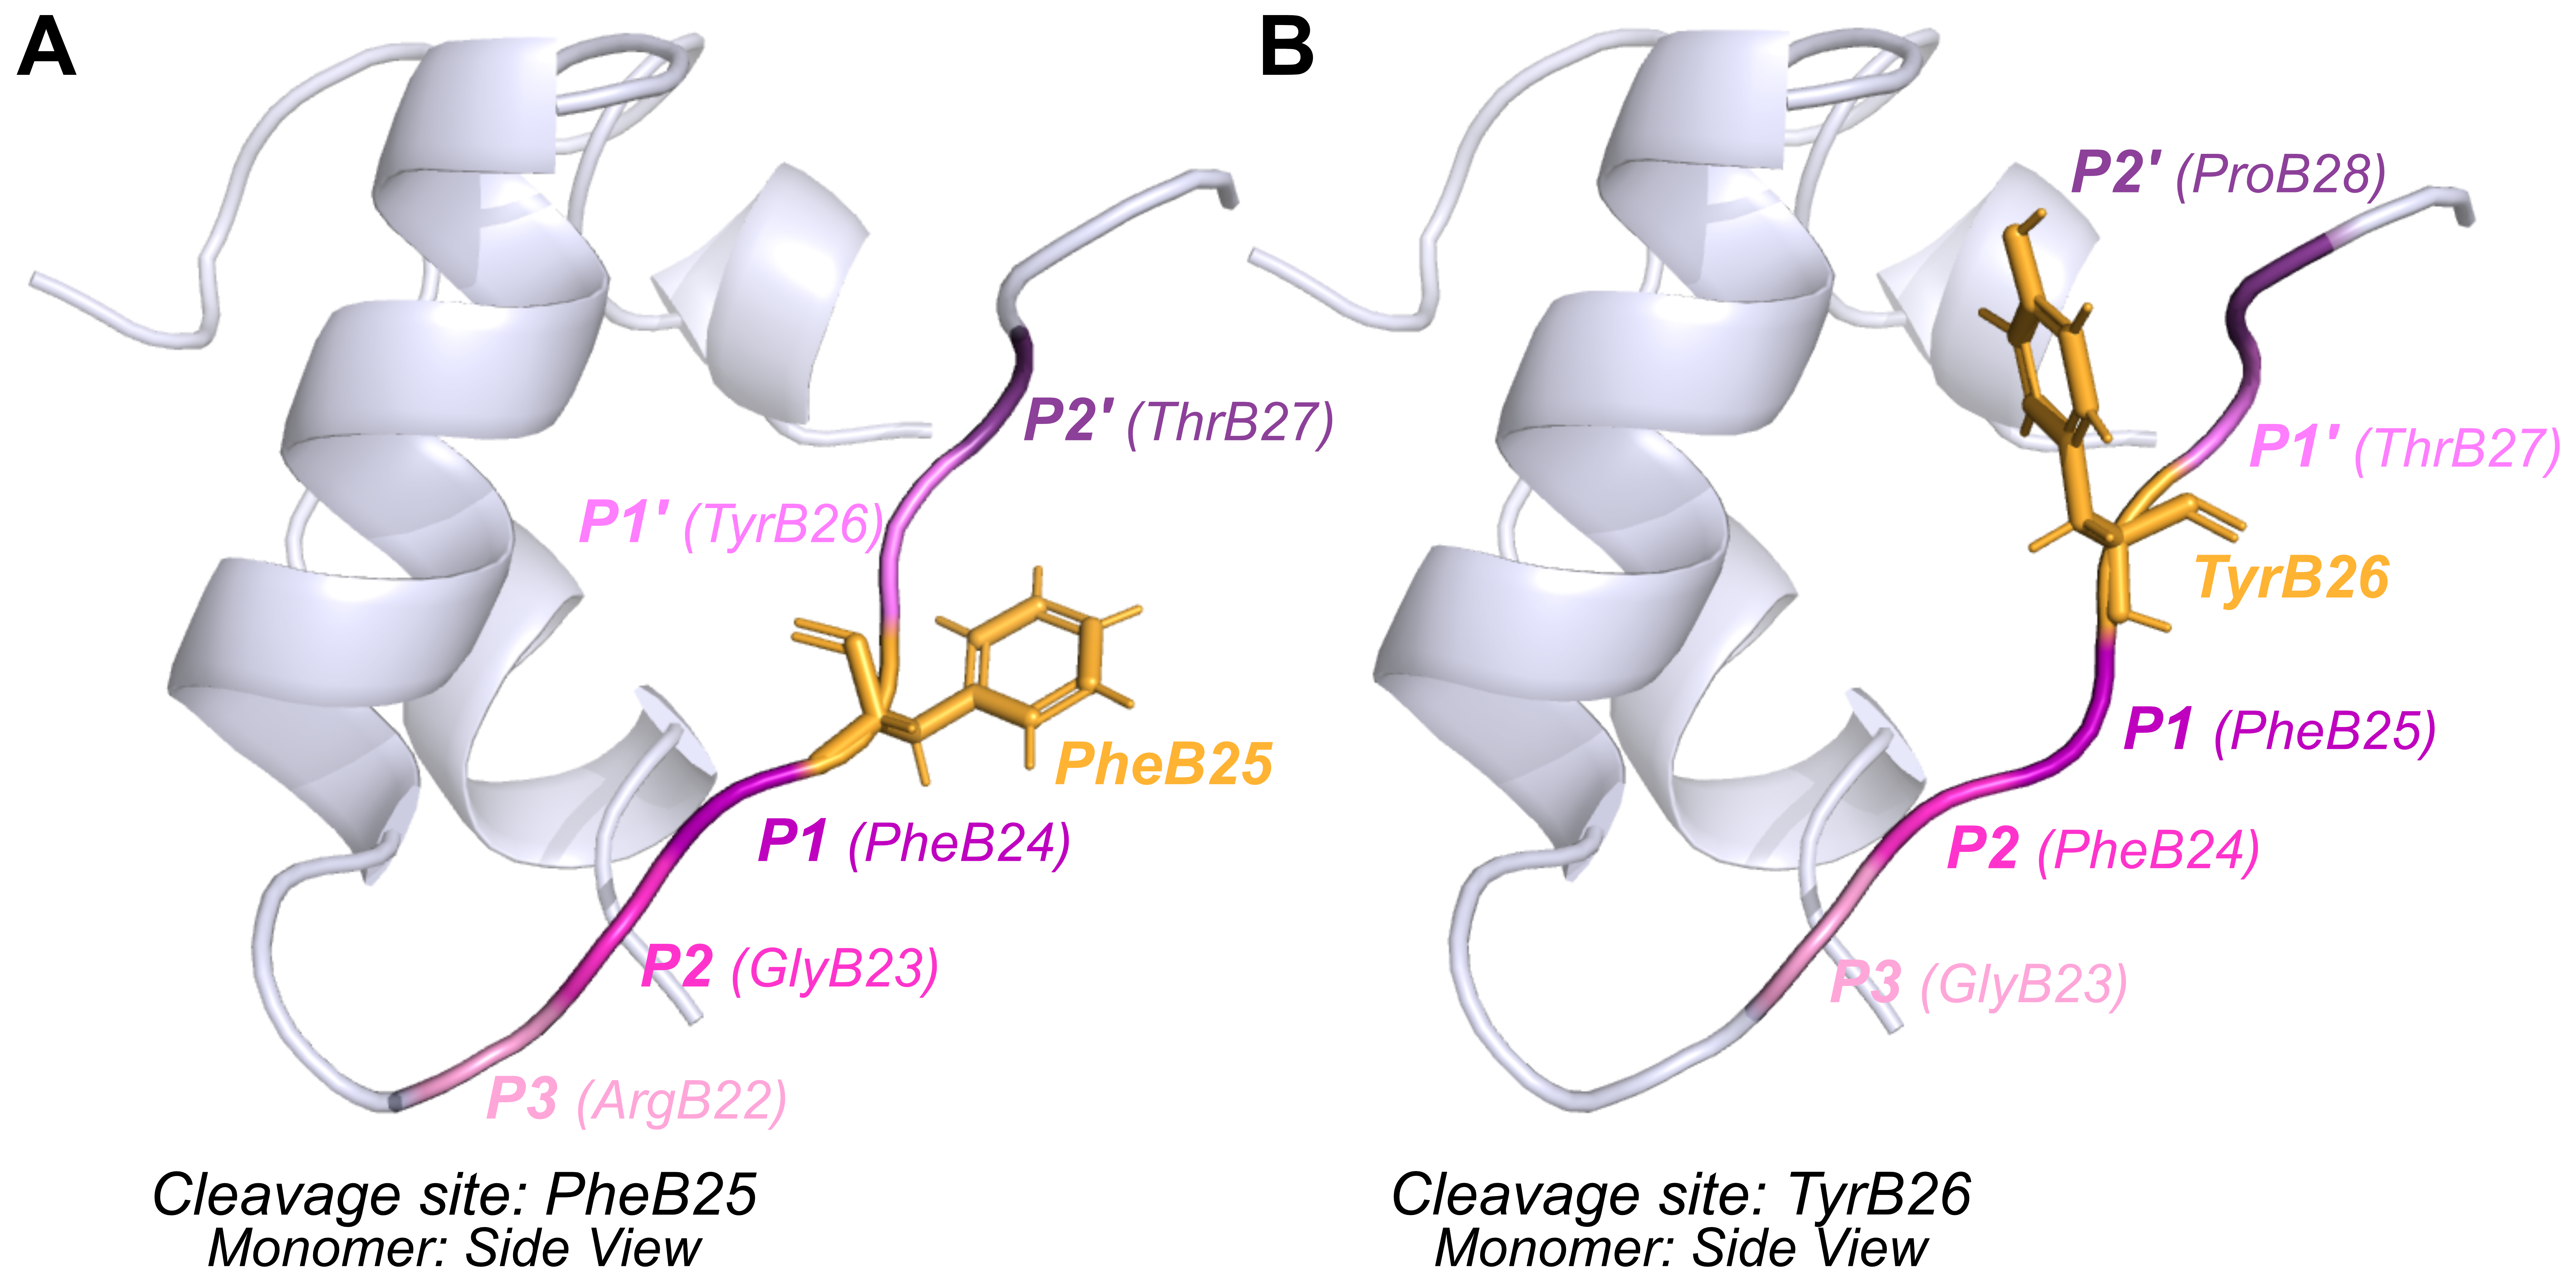
\includegraphics[width=0.95\textwidth]{Figures/P_sites.png}
\caption{The P- and P'-sites of the two most important cleavage sites, residues PheB25 and TyrB26. The cleavage sites are shown as  orange sticks, while the remaining part of the protein is shown in cartoon representation. Schechter-Berger nomenclature for residues surrounding the cleavage sites are shown in varying shades of magenta and are labeled P1-3 and P1'-2'.}
\label{P_sites}
\end{figure}

\paragraph{Metric 4: Existence of glycan-involved hydrogen bonds}
In addition to the consensus conformations of the binding sites, some of the hydrogen bonds between $\alpha$-chymotrypsin and the substrate were also found crucial for efficient substrate hydrolysis~\cite{hedstrom2002serine}. These hydrogen bonds include the ones involved in the antiparallel $\beta$-sheet, formed between (1) the carbonyl oxygen of Ser214 and the amide NH of the P1 site, (2) the amide NH of Gly216 and the carbonyl oxygen of the P3 site, and (3) the carbonyl oxygen of Gly216 and the amide  NH of the P3 site. Additionally, the main-chain carbonyl oxygen of Phe41 also forms a hydrogen bond with the amide NH of the P2' site. These four hydrogen bonds in the P3'--P3 region are commonly believed to form the canonical hydrogen-bonding network between insulin and $\alpha$-chymotrypsin. With this in mind, we hypothesized that the oxygen atoms of the glycan could compete with the $\alpha$-chymotrypsin residues (Ser214, Gly216, and Phe41) as the acceptors to form hydrogen bonds with insulin residues (the P1-P3 sites, and the P2' site), hence disturbing the hydrogen-bonding network and potentially enhancing the proteolytic resistance of the structure. To see what additional interactions were formed due to the presence of the glycan, we examined all the glycan-involved hydrogen bonds, not just the ones involving the P1-P3 and P2' residues. We used MDtraj~\cite{mcgibbon2015mdtraj} to identify hydrogen bonds between the glycan moiety (as the acceptor) and any insulin residue (as the donor) according to the Baker-Hubbard criterion~\cite{baker1984hydrogen}, which identified a hydrogen bond only if the angle formed between the donor, hydrogen atom and the acceptor was larger than 120 degrees and the distance between the hydrogen atom and the acceptor was less than 2.5 angstrom at least 10\% of the time. For each trajectory, we calculated the fraction of the time each hydrogen bond existed and averaged the fractions of the hydrogen bonds of each glycoform across the 5 different wild-type bases. The ones whose fraction is larger than 5\% are reported, with the uncertainty being the standard deviation.

\subsubsection{Dimerization Propensity}
The dimerization propensity metric was compared to experimental dimerization data from Guan et al.~\cite{guan2018chemically}. Dimerization data exists only for wild type, GF 9, GF 10, and GF 13, and thus comparisons between experimental and computational data proved challenging. We focused only on residues GlyB23--TyrB26 because these are the dimer interface residues that form backbone hydrogen bonds with another insulin monomer (Figure \ref{starting_structures}B)~\cite{timofeev2010x, harding1966crystal, antolikova2011dimerinterface}. 

One potential signature of dimerization propensity is the presence of dimer-characteristic structure in the monomer ensemble, which would reduce the free energy of reorganization on dimerization. However, we found no consistent secondary structure propensity differences in either the dimer or the monomer between glycoforms or between glycoforms and the wild type. This was also true after examining additional monomer structures 1JCO~\cite{keller2001flexibility}, 1MHJ~\cite{jorgensen1996solution}, and 2JV1~\cite{bocian2008structure}. This suggests to us that such structural analysis alone of glycoforms will not allow us to determine dimerization propensity, and so we explored different metrics to assess dimerization.
\paragraph{Metric 1: Glycan-dimer occlusion}
We considered steric occlusion of the dimer interface by the glycans as a possible metric for dimerization. Several glycan moieties are attached close to the explicit dimerization region GlyB23--TyrB26 (Figure \ref{sys_of_interest}), and there are several glycans large enough to sterically interfere with the dimerization interface (Figure \ref{occlusion}). We hypothesized that glycans that occupy space close to these residues, with high frequency in simulation time, will preclude dimerization.

We defined glycan-dimer occlusion as any instance when at least one atom of the glycan moiety comes within 5 angstroms of any atom in the dimer interface GlyB23--TyrB26, including the atoms in the backbone and in the side chains. We used the Python package ProDy~\cite{bakan2011prody} to calculate the total number of atom neighbor pairs between the glycan and dimer interface for each frame in the trajectories.

Atom neighbor pair autocorrelation lag times (in ns) were estimated by fitting autocorrelation data to an exponential decay function using SciPy~\cite{scipy2020pub, numpy2020pub} and are presented in Supplemental Table S4. There are several glycoform models that have no lag time ("NA" in Supplemental Table S4) and this is because for these trajectories, no occlusion was found. The lag times were used to estimate the independent occlusion states sampled throughout the simulation by dividing the total simulation time by the subsequent lag times.

To simplify the occlusion analysis, we calculated the proportion of simulation frames that contain a glycan-dimer atom neighbor pair out of the total simulation frames, and ignored the absolute number of atom neighbor pairs in each frame so as to treat any number of interactions as possible occlusion. Since larger glycans will have more possible neighbors than smaller glycans, this also served to normalize the data to prevent a bias for the larger glycans. The 95\% confidence intervals for these binomial proportions were estimated using the independent occlusion samples and the Wilson score method, which produces bounded asymmetric intervals and does not require normal approximations for its use~\cite{wilson1927score, newcombe1998intervals, wallis2013binomialscores}. The proportion of frames with occlusion for each glycoform were only compared within its respective set, because no wild-type control could be included as the wild type is not glycosylated.

\begin{figure}[H]
\centering
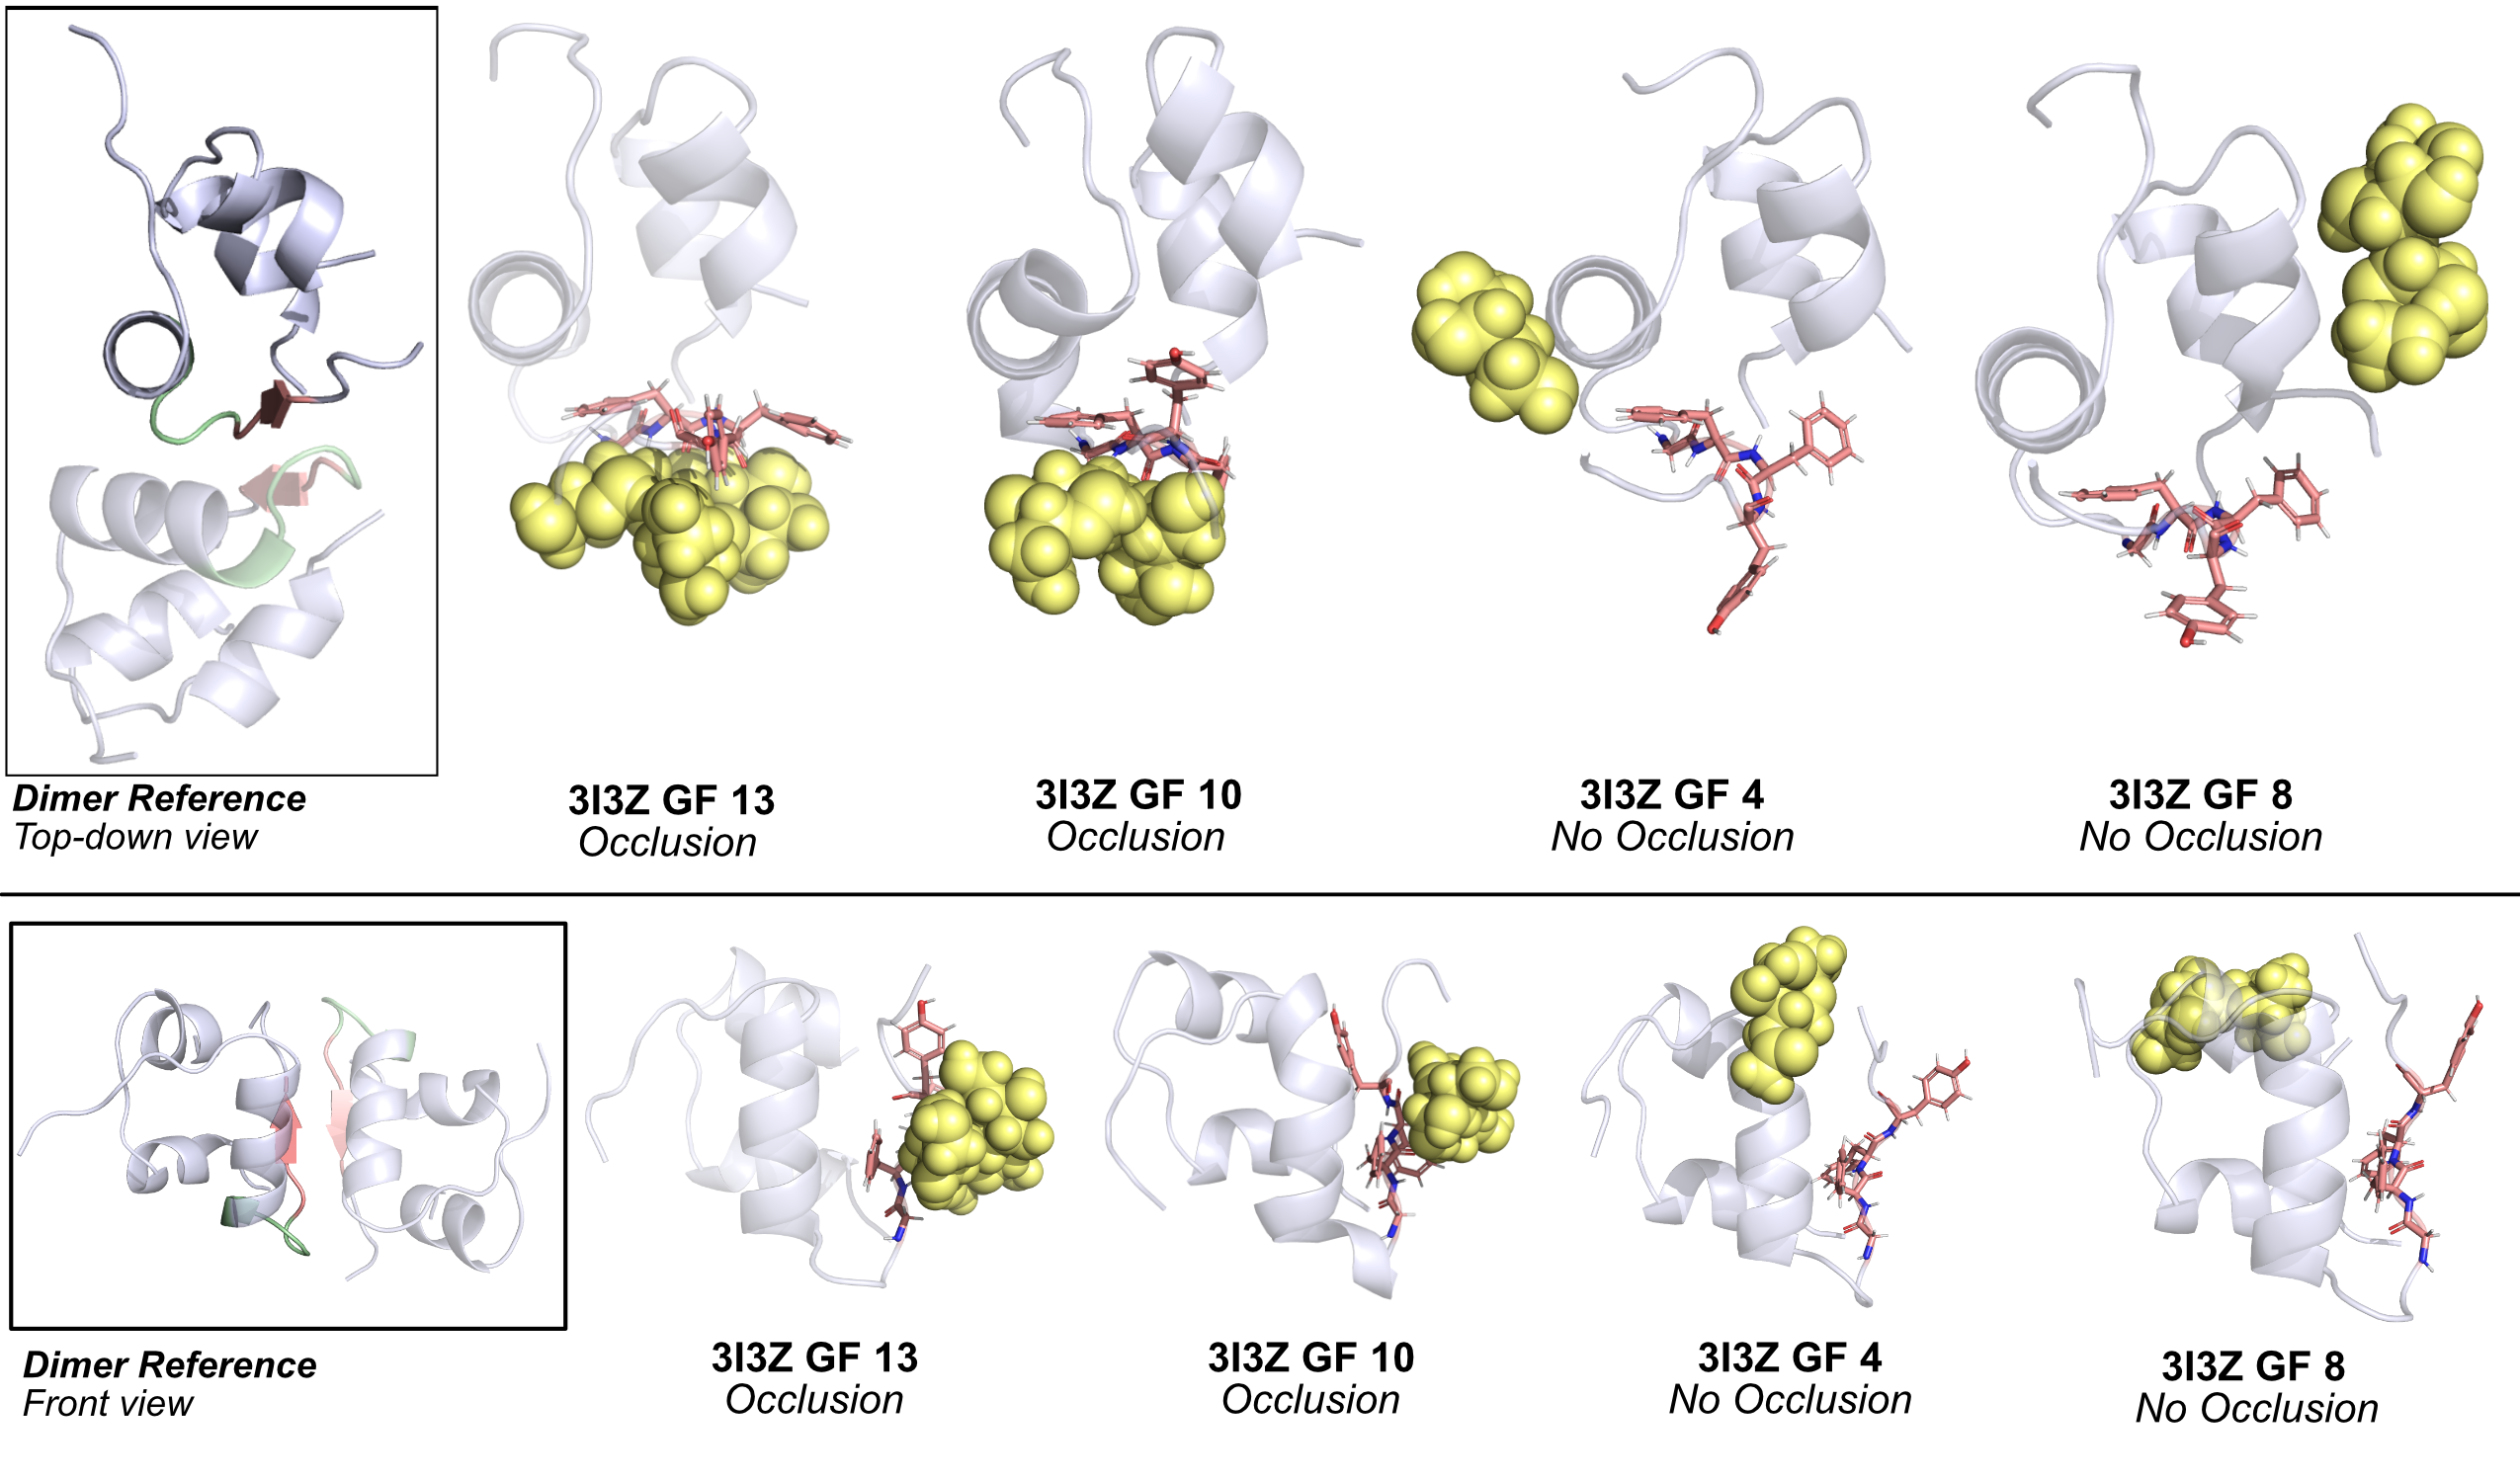
\includegraphics[width=\textwidth]{Figures/Fig_dimer_occlusion.png}
\caption{Classification of occlusion and no-occlusion states. Representative frames from four different glycoform trajectories show occlusion (GF 13, GF 10) and no occlusion (GF 4, GF 8) states. Insulin monomer is presented in translucent blue-white cartoon, dimerization residues presented in salmon sticks, and glycan moiety presented in yellow spheres. The 3I3Z dimer structure is provided as the reference.}
\label{occlusion}
\end{figure}

\subsection{Bootstrap methods for estimating the uncertainties of correlation coefficients} \label{bootstrap}
In the correlation plots presented in both the main text and the supporting information, we performed bootstrapping to estimate the uncertainties of correlation coefficients. 

Specifically, in the main text, all the correlation plots characterize the relationship between one metric and the experimental data. Therefore, in each of the 500 bootstrap iterations we performed, for each variant, we drew five bootstrap samples for value of the metric from the set of five different wild-type models, and five bootstrap samples for the experimental reference from normal distributions centered at the experimental values. From each of these 500 bootstrap iterations, we calculated one Kendall's tau correlation coefficient by correlating the sample mean of the two variables. Lastly, we calculated the standard deviation of these 500 values and reported it as the uncertainty of the correlation coefficient. 

The same bootstrap method was used to estimate the uncertainty of the Pearson correlation coefficients annotated in Supplemental Figure S3 to S5, except that the bootstrap samples for both metric variables of interest were drawn from values based on different wild-type models.

\subsection{Molecular Visualization}
Molecular visualization, specifically for Figure \ref{sys_of_interest}, \ref{starting_structures}, \ref{P_sites}, \ref{occlusion}, and S6, were done using PyMOL version 2.4.1~\cite{delano2002pymol}.

% %===============================
% % Results and Discussions
% %===============================
\section{Results and Discussions}\label{results}
\subsection{Proteolytic degradation}
\subsubsection*{Metric 1: SASA of scissile bonds}
According to our hypothesis of the peptide bond SASA of the cleavage sites, glycoforms whose scissile bonds are less solvent-exposed should have higher proteolytic stability. To examine this hypothesis, we plotted the $\alpha$-chymotrypsin half-life measured in the experimental work against the SASA value of each of the two scissile bonds, including the one between residues B25 and B26 (upper panel of Figure \ref{result_sasa}A) and the one between residues B26 and B27 (lower panel of Figure \ref{result_sasa}A). Ideally, a good computational metric should be able to reproduce consistent results as compared to the work by Guan et al.~\cite{guan2018chemically}, leading to a Kendall's tau correlation coefficient close to -1. A good metric should also be immune to the starting model bias, including the bias from wild-type models resolved using different methods or under different conditions, or the bias solely from different protonation states of the histidine residues. 

As a result, we conclude that the SASA of the scissile bonds is a weak predictor for proteolytic stability. GF 13 and GF 10, which were experimentally found to be more proteolytically stable than the wild type, did have a lower SASA value than the wild type at both sites. Notably, as the most proteolytically stable structure, GF 13 also had the lowest SASA values at both sites. However, GF 10 had the second-longest $\alpha$-chymotrypsin half-life, but not the second-lowest SASA values at both sites. At the scissile bond between B26 and B27, most glycoforms had a lower SASA value than that of the wild type, but some of them were experimentally identified as less proteolytically stable than the wild type. Overall, the SASA values of either scissile bond have roughly the same efficacy given similar values of Kendall’s tau correlation coefficients. However, if we are only interested in the comparison between the wild type and any glycoform instead of between any two of the glycoforms, the SASA value of the scissile bond between B25 and B26 is marginally more indicative than the SASA value of the other site. Specifically, among all the glycoforms that had shorter $\alpha$-chymotrypsin half-lives than the wild type, GF 3, GF 4, GF 7, and GF 8 indeed had higher SASA values at this site than the wildtype. As for GF 6 and GF 11, which also had short $\alpha$-chymotrypsin half-lives than the wild type, the SASA value at the B25-B26 scissile bond failed to classify them as the less proteolytically stable variants. Notably, the errors in the metric are generally large, which might be attributable to the fact that the SASA of the scissile bond was calculated from only 4 atoms (CONH atoms) and could lead to larger fluctuations in nature. Regardless of whether these large error bars are a direct result of the dependence of the initial bias or not, this high uncertainty undermined the predictiveness of this metric, making it less useful.

\begin{figure}[H]
\centering
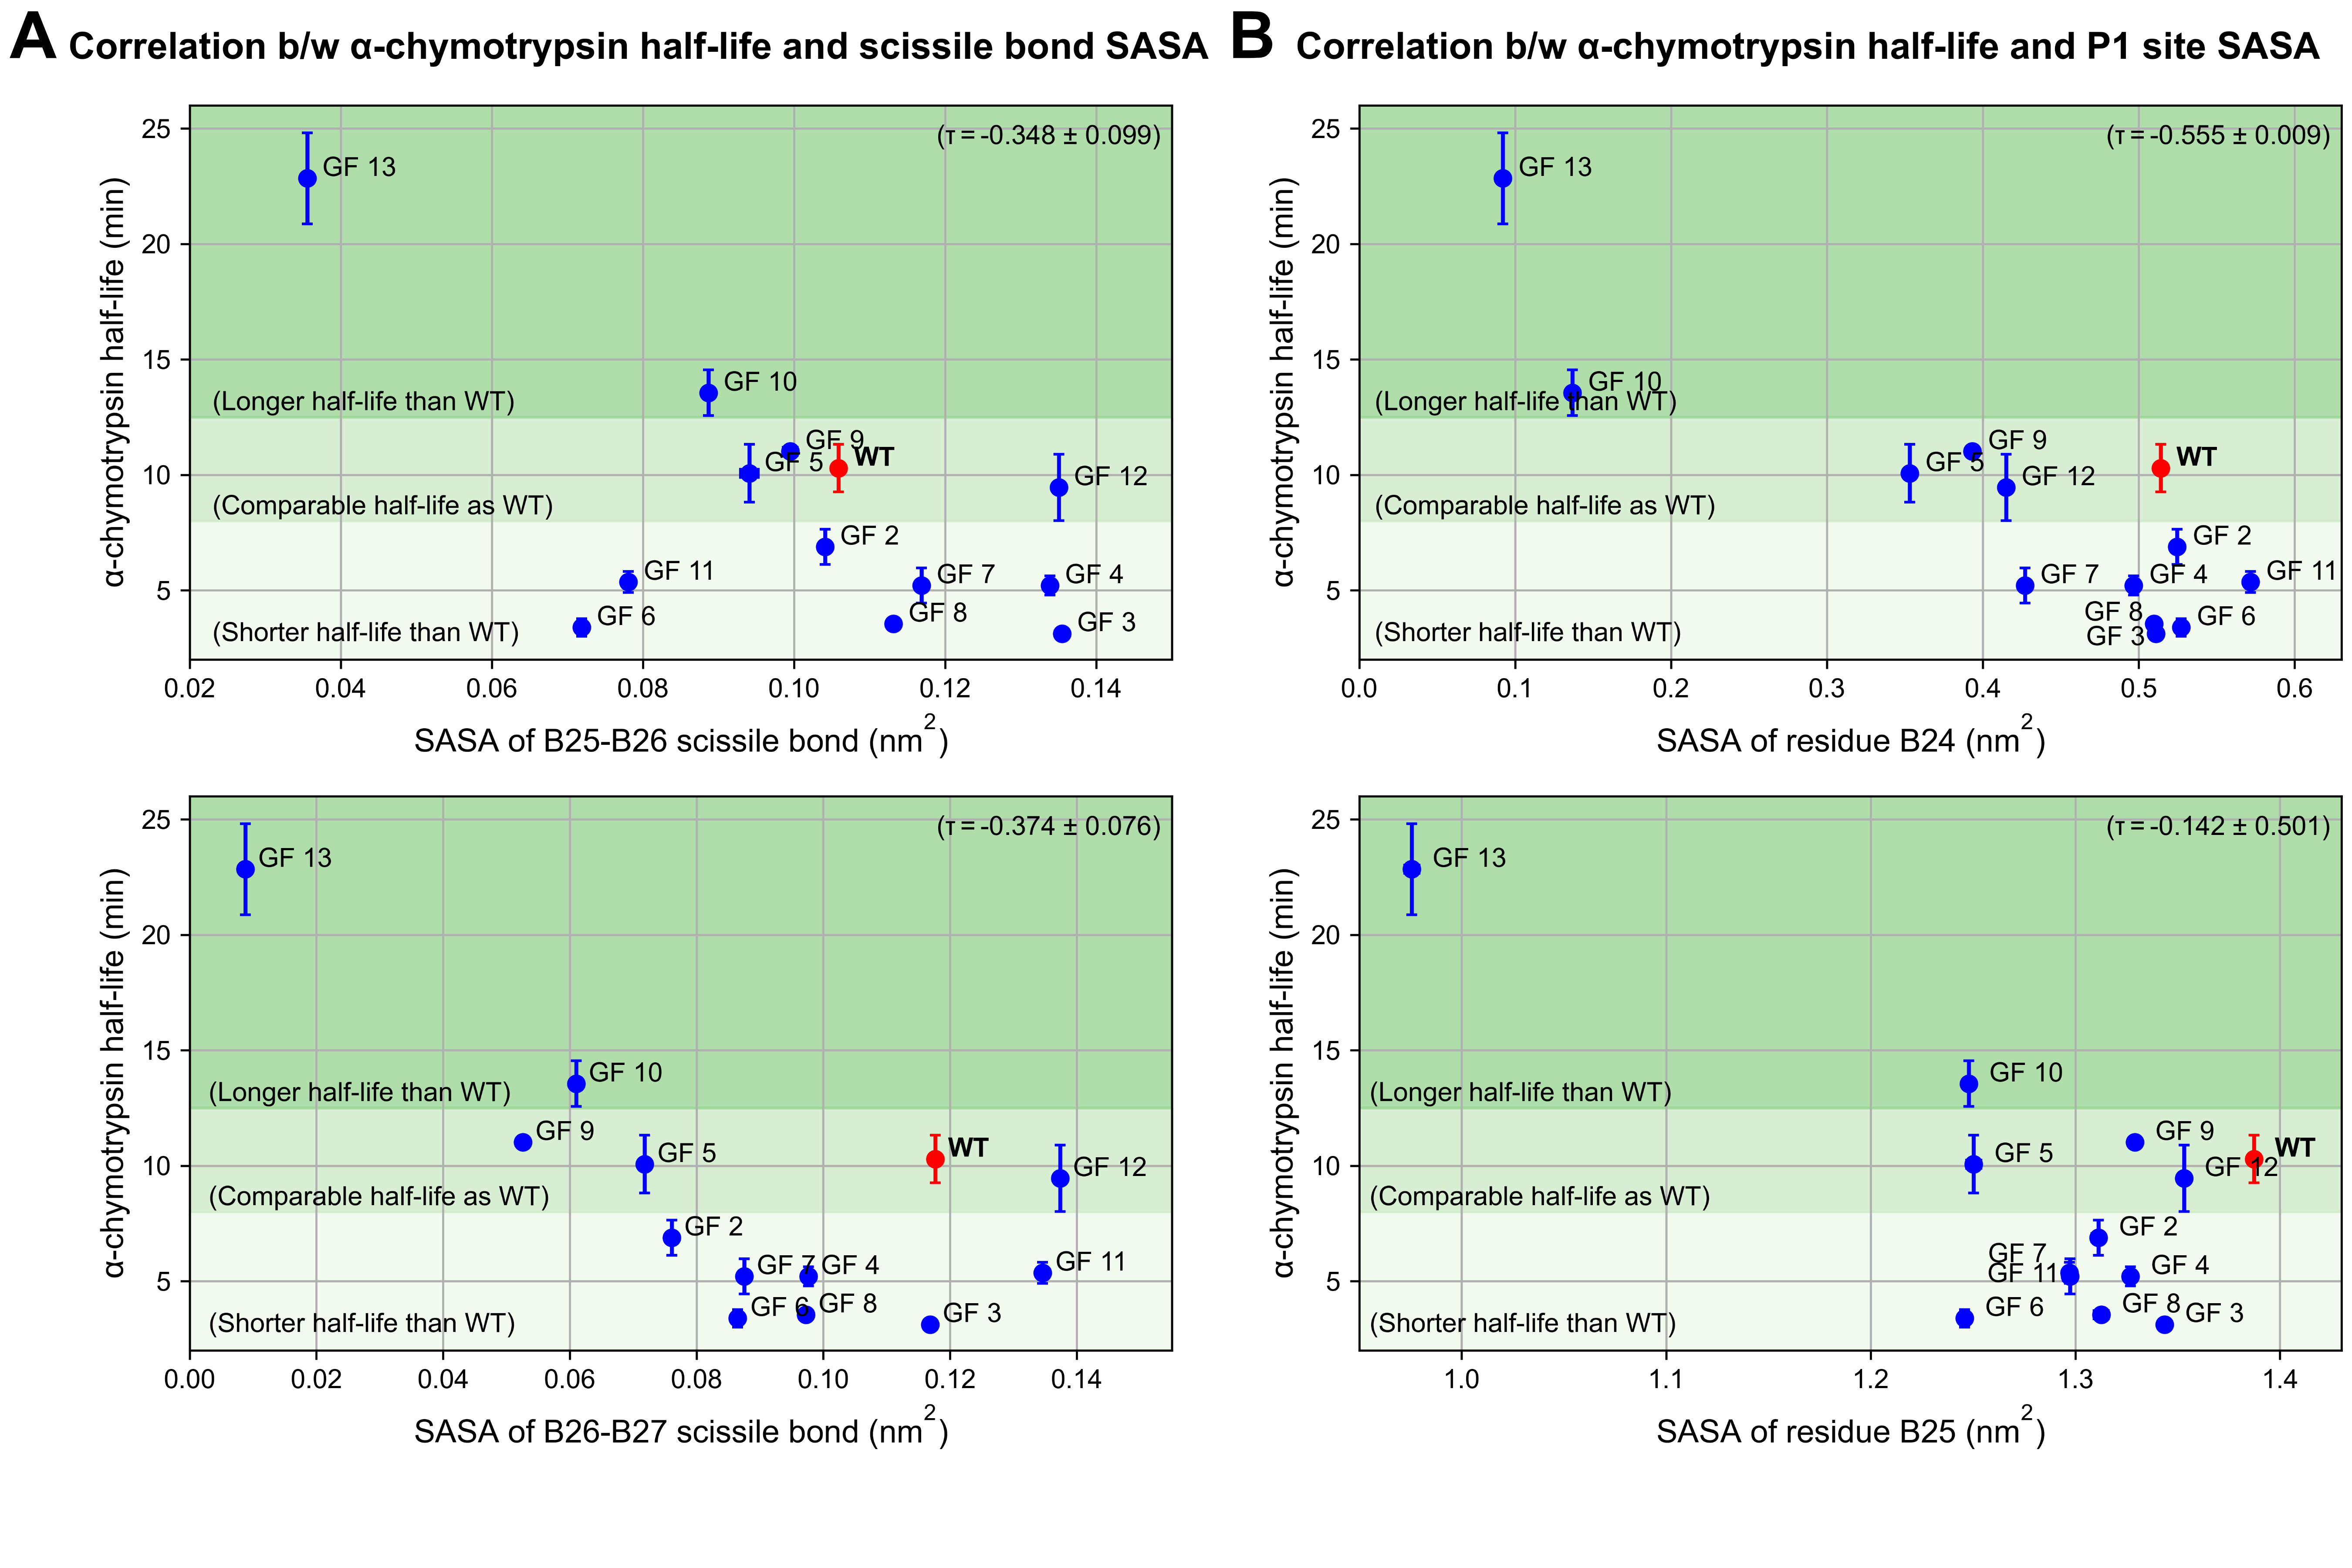
\includegraphics[width=\textwidth]{Figures/Fig_SASA_correlation.png}
\caption{The SASA of both the scissile bonds and the P1 sites are weakly correlated with $\alpha$-chymotrypsin half-life, implying moderate predictiveness for the proteolytic stability. (A) The correlation plot between the $\alpha$-chymotrypsin half-life and the average SASA of the scissile bonds in the glycoforms (GF). (B) The correlation plot between the $\alpha$-chymotrypsin half-life and the average SASA of the P1 sites in the glycoform (GF). Different regions were colored to indicate glycoforms having longer, comparable, or shorter half-life as compared with the wild type. The Kendall's tau correlation coefficient ($\tau$) and its uncertainty were calculated. Error bars of both variables are shown. The distributions of the data are provided in Supplemental Figure S2.}
\label{result_sasa}
\end{figure}

\subsubsection*{Metric 2: SASA of the P1 sites}
Similar to Metric 1, Metric 2 is partially predictive and has relatively large error bars for some of the variants. 

In the lower panel of Figure \ref{result_sasa}B, the SASA of residue B25 is less predictive than the SASA of the other site. Although an agreement with experimental results can be seen from GF 13, which had the lowest SASA at residue B25 and was previously found to be the most proteolytically stable, other glycoforms, regardless of the $\alpha$-chymotrypsin half-life, all had a lower value compared to the wild type. The Kendall's tau correlation coefficient, which was close to 0, shows that the SASA of residue B25 was almost uncorrelated with the $\alpha$-chymotrypsin half-life. 

The SASA of residue B24 (the upper panel of Figure \ref{result_sasa}B), on the other hand, had a higher correlation with the proteolytic stability of the structure. Specifically, GF 13 and GF 10, the two most proteolytically stable glycoforms, had significantly lower SASA value at residue B24. As for the glycoforms that had a lower SASA value at this site, except for GF 7, all had comparable proteolytic stability to the wild type. This higher correlation can also be seen from the magnitude of the corresponding Kendall's tau correlation coefficient, which was higher than those of Metric 1.

Overall, these observations imply moderate predictiveness of the SASA of residue B24, since a low value at this site generally indicates that the structure is very likely to have more, or at least comparable proteolytic stability compared to the wild type. Notably, most proteolytically unstable glycoforms, including GF 2, GF 3, GF 4, GF 6, GF 7, and GF8, had the same level of SASA at residue B24 as the wild type. This could be attributable to the situation where the residue of the wild type is already very solvent-exposed, leaving considerably less space for the proteolytically unstable glycoforms to have an even higher SASA value. This limitation is intrinsic to both Metric 1 and Metric 2, motivating us to look for more reliable predictors for proteolytic stability. 

\subsubsection*{Metric 3: \texorpdfstring{$\beta$}{Lg}-sheet propensity of the P1--P3 region}
Our hypothesis suggests that glycoforms whose P1--P3 region has a lower $\beta$-sheet propensity should potentially have higher proteolytic stability. However, most of the residues, including B22, B23, and B24 did not show this trend, while residue B25 did show predictiveness of roughly the same level as Metric 1 since it showed the lowest $\beta$-sheet propensity for the most proteolytically stable structures (GF 10 and GF 13). Notably, even if one of the four residues exhibited moderate predictiveness, the generally large error bars in the $\beta$-sheet propensity undermine its usage as a metric to capture structural determinants that influenced the proteolytic stability of the structure. These large error bars in the case of B22 to B24 also imply that the structure at these sites can adopt a wide range of orientations, contradicting our hypothesis that the glycoforms able to prevent proteolytic degradation should have common orientations at these sites due to high free energy costs of structural re-orientations or transformations. Similar to the first two metrics, we note that these large error bars are not necessarily the results of the starting model bias, since the $\beta$-sheet propensity was calculated from the orientations of just a few atoms, which naturally caused larger fluctuations of the results. Since the metric is insufficient to assess the proteolytic stability, whether or not the large error bars can be ascribed to the starting model bias is not relevant. 


\begin{figure}[H]
\centering
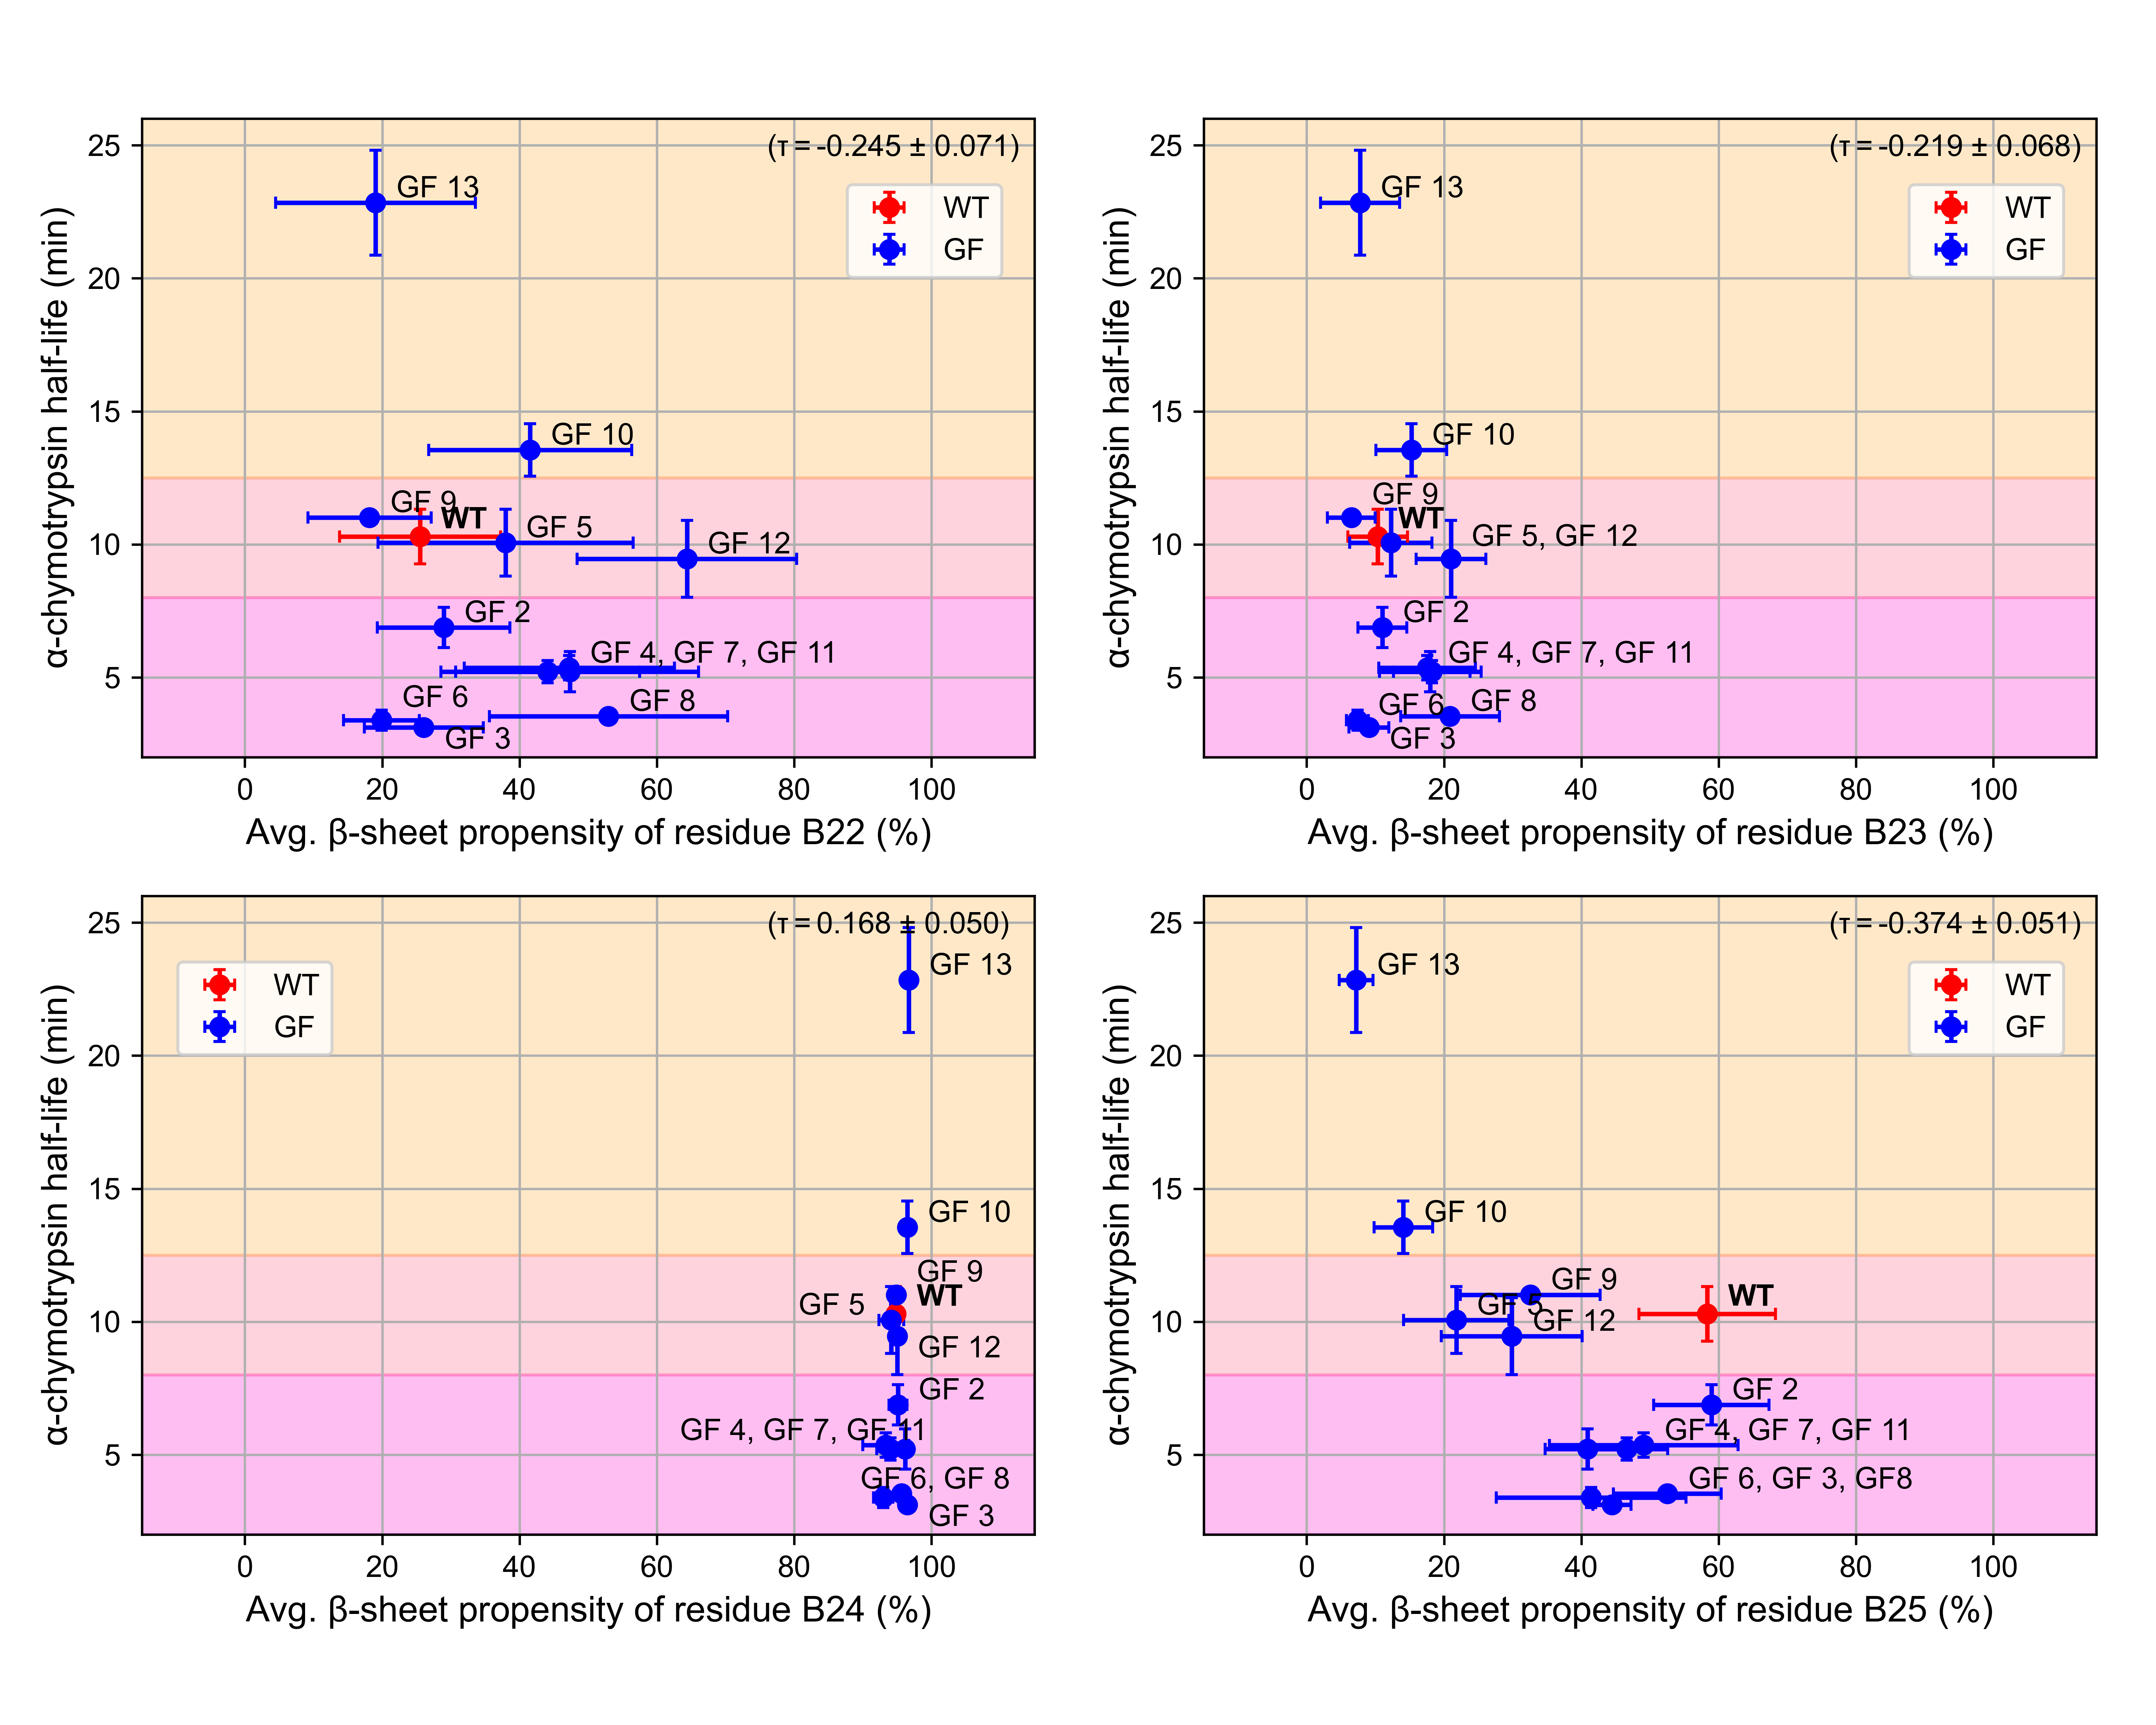
\includegraphics[width=\textwidth]{Figures/avg_beta_propensity_correlation.png}
\caption{The correlation plot between the $\alpha$-chymotrypsin half-life and the average $\beta$-sheet propensity of residues B22 to B25. The $\beta$-sheet propensity of the P1-P3 region does not correlate with $\alpha$-chymotrypsin half-life. Different regions were colored to indicate glycoforms having longer, comparable, or shorter half-life as compared with the wild type. The Kendall's tau correlation coefficient ($\tau$) and its uncertainty were calculated. Error bars of both variables are shown.}
\label{result_beta}
\end{figure}

\subsubsection*{Metric 4: Existence of glycan-involved hydrogen bonds}
We hypothesized that glycoforms with more glycan-involved hydrogen bonds, especially the ones that involved the P1--P3 or the P2' sites, could interfere with the canonical hydrogen-bonding network formed between the protease and the substrate, thus enhancing the proteolytic stability of the substrate. This metric does turn out to be in large part predictive of proteolytic stability of the glycoforms. 

Figure \ref{result_hbond} shows the percentage of the time each kind of hydrogen bond existed in the MD simulations. As a result, proteolytically stable glycoforms such as GF 13 and GF 10 had the most glycan-involved hydrogen bonds. Glycoforms with comparable proteolytic stability as the wild type, including GF 5, GF9, and GF 12 had at least one or two glycan-involved hydrogen bonds. Most of the remaining glycoforms, which were more susceptible to proteolytic degradation than the wild type, had no glycan-involved hydrogen bonds. Importantly, glycoforms having at least comparable proteolytic stability as the wild type typically have hydrogen bonds that involved residues PheB24 or ThrB27, which were the P1 site and the P2' site corresponding to the cleavage site B25, respectively. In glycoforms that had an intermediate level of proteolytic stability (GF 5, and GF 9), hydrogen bonds involving these two residues were not present or at least not long-lasting in the MD trajectories (see Supplemental Table S5), as reflected by the large errors bars that almost reached the bottom of the graph. On the other hand, in the proteolytically stable glycoforms, GF 13 and GF 10, hydrogen bonds ThrB27(N)--Man[2](O6) and PheB24(N)--Man[1](O3) were found in all GF 13/GF 10 MD trajectories, regardless of which wild-type model the glycoform was built on. We concluded these two kinds of hydrogen bonds (ThrB27(N)--Man[2](O6) and PheB24(N)--Man[1](O3)), the longest-lasting glycan-involved hydrogen bonds in the most proteolytically stable structures, were the most important hydrogen bonds influencing the proteolytic stability in our study. Interestingly, GF 13 occasionally had a hydrogen bond formed between ThrB27 and the third mannose, which was absent from GF 10. This additional hydrogen bond that involved a P2' site might further interfere with the hydrogen bonding network between insulin and $\alpha$-chymotrypsin, making GF 13 even more proteolytically stable than GF 10. 

Overall, the predictions made out of the glycan-involved hydrogen bonds analysis are relatively consistent with the experimental results. The only exception is GF 6, which was experimentally found to be less proteolytically stable than the wild type but had a hydrogen bond, ThrB27(N)-GalNAc[1](O3) that involved a P2' site ThrB27. However, this hydrogen bond was only present in the MD trajectories of 4EYD-, 4EY1-, and 2MVC-based GF 6 (see Supplemental Table S5), indicating that this hydrogen bond might not be stable enough to consistently disturb the aforementioned hydrogen bonding network. Importantly, the fact that 4EYD-, 4EY1-, and 2MVC-based GF 6 all possess the same hydrogen bond is one of many examples showing the large error bars should be irrelevant to the initial modeling bias. Specifically, if there is a bias from the differences in the resolution methods or the histidine protonation states, glycoforms resolved by the same method (e.g. 4EYD-, 4EY9-, and 4EY1-based glycoforms) or having the same histidine protonation states (e.g. 4EYD-, 4EY1- and 3I3Z-based glycoforms) should exhibit similar hydrogen bond distributions at the examined site. However, this trend is absent from our results, suggesting that the metric is independent of the starting wild-type models. Finally, we can conclude that long-lasting, stable glycan-involved hydrogen bonds, especially the ones that involve PheB24 and ThrB27, appear critical in enhancing the proteolytic stability of the structure. This conclusion also underpins the findings in the work by Guan et al.~\cite{guan2018chemically} that ThrB27 and ThrB30 were identified as the best two glycosylation sites, as the glycan attached to these sites are structurally closer to the important residues (ThrB27 and PheB24) found in this study. 
\begin{figure}[H]
\centering
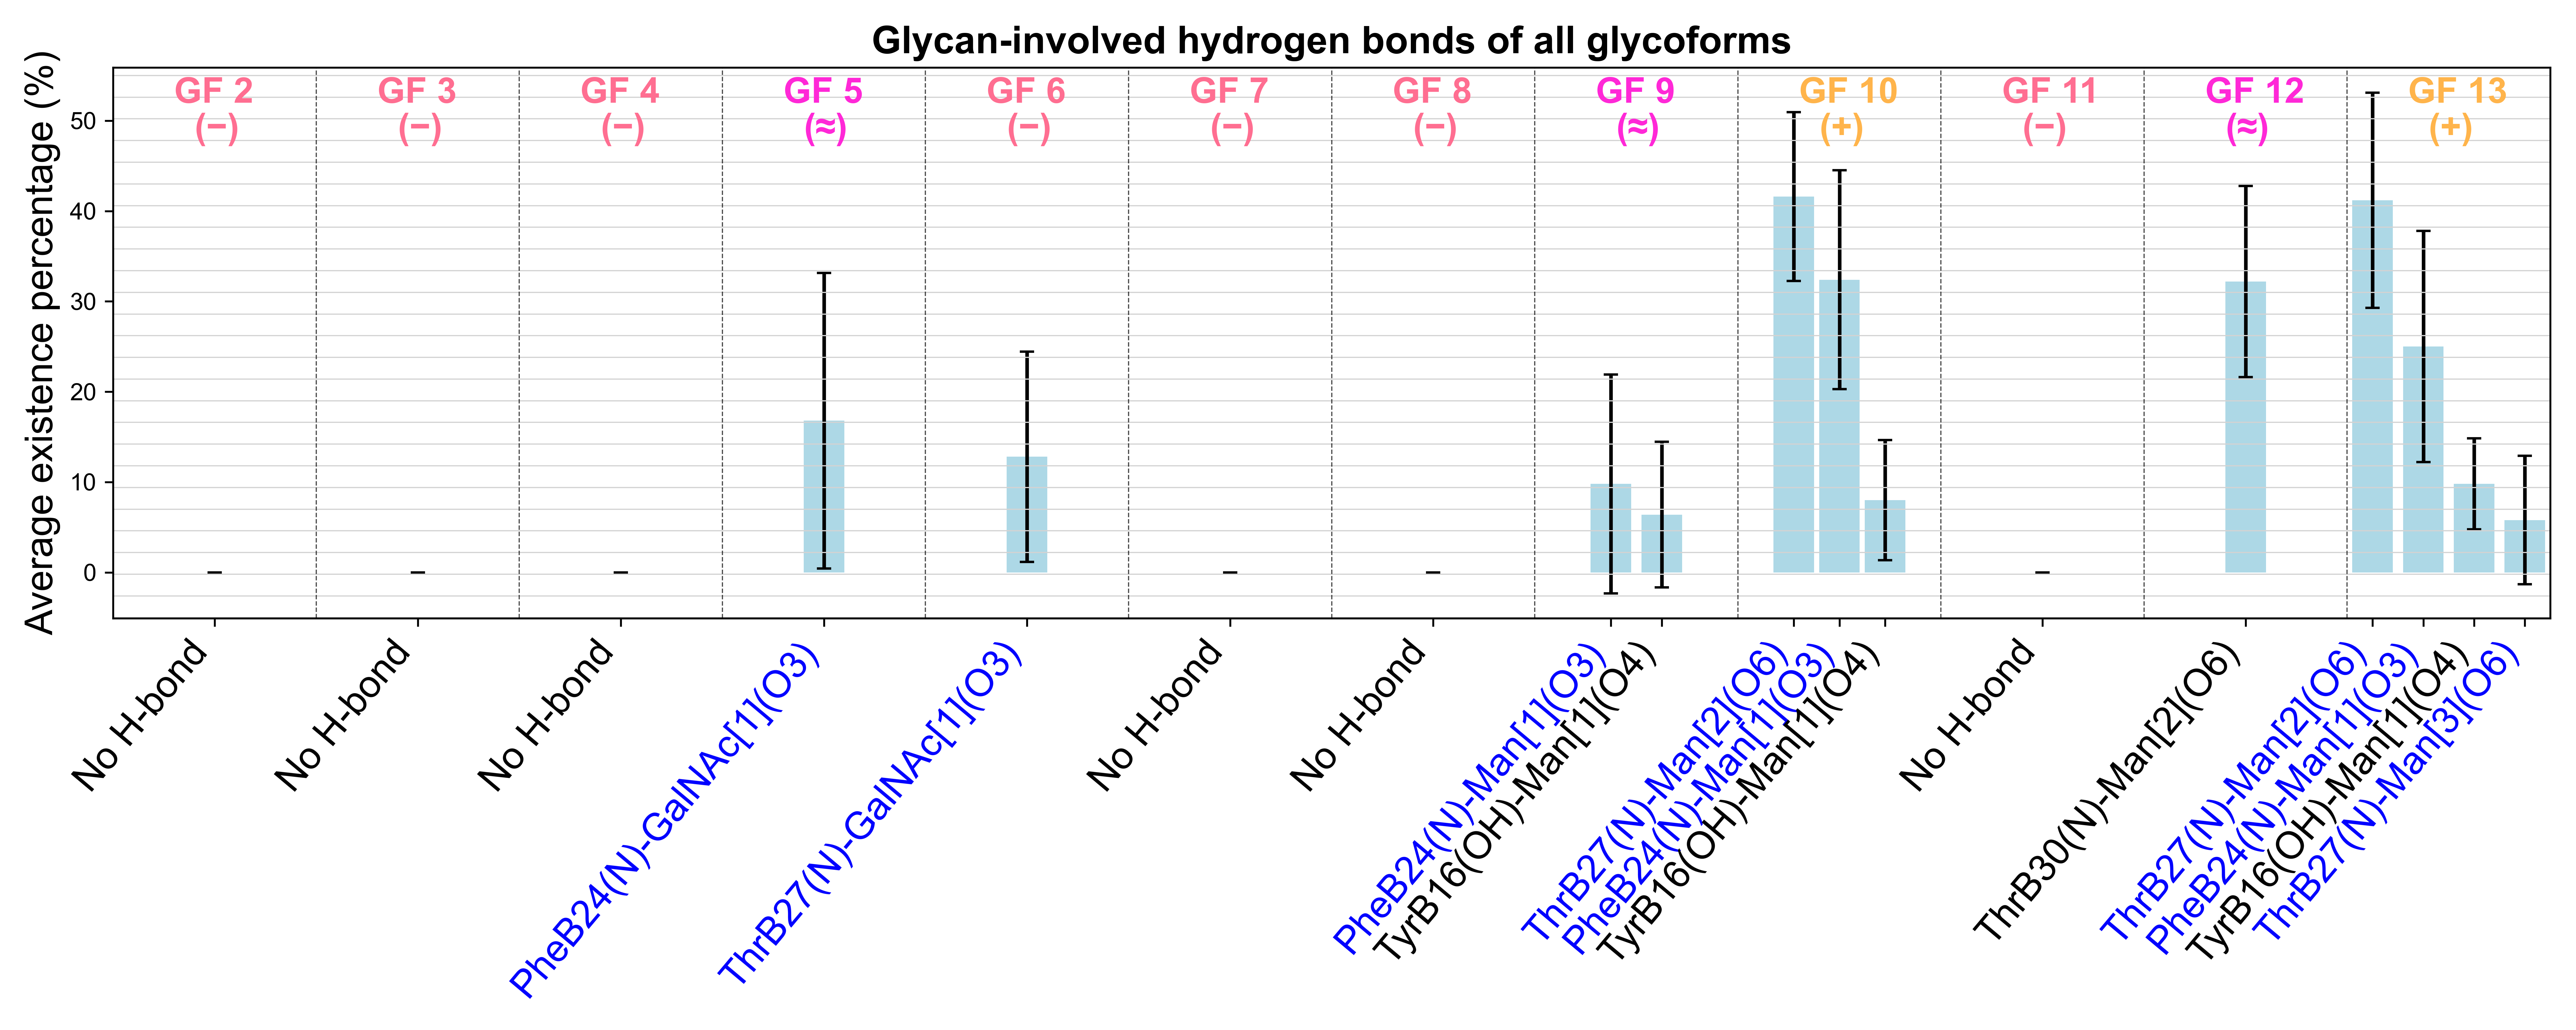
\includegraphics[width=\textwidth]{Figures/hbond_results.png}
\caption{The most proteolytically stable glycoforms tend to have more glycan-involved hydrogen bonds, especially the ones involving the residues PheB24 and ThrB27. The figure shows the percentage of the time each kind of hydrogen bond existed in the MD simulations. The experimental results are summarized such that $+$(yellow), $-$(red), and $\approx$(magenta) respectively indicate that the corresponding glycoform was experimentally found to have higher, lower and comparable proteolytic stability as compared to the wild type. Note that in the name of each hydrogen bond, the 1-based index of the glycan is shown in the bracket following the name of the glycan. The atom type is shown in the parenthesis right after the residue name. (See Supplemental Table S6 for more details of the atom types shown in the figure.) For example, ThrB27(N)--Man[2](O6) means the hydrogen bond formed between the amide N atom of ThrB27 as the donor and one of the oxygen atoms of the second mannose as the acceptor. Texts for hydrogen bonds that involve any of the P1--P3 or the P2' residues are colored in blue, which in our case only include PheB24 and ThrB27.}
\label{result_hbond}
\end{figure}

\subsection{Dimerization Propensity}
\subsubsection{Metric 1: Glycan-dimer occlusion}
Based on our dimerization hypothesis, glycoforms whose glycans come in proximity to the dimer interface (GlyB23--PheB26) will be less prone to dimerize because of steric occlusion by the glycan. We found that this glycan-dimer occlusion might be a useful predictor of dimerization propensity. 

To test this hypothesis, we calculated the glycan-dimer occlusion metric for each glycoform and considered those with low occlusion to have high dimerization propensity, and vice versa. Figure~\ref{occlusion} shows representative frames from four 3I3Z trajectories to visually demonstrate occlusion versus no-occlusion, where the light blue cartoon represents insulin, salmon sticks represent residues GlyB23--PheB26, and pale yellow spheres represent the glycan moiety. 

Using the glycan-dimer occlusion metric, we calculated the proportion of simulation frames with occlusion for each glycoform and ordered them from least occlusion to most occlusion, shown in Supplemental Table S7. We must carefully compare these results to experimental dimerization data~\cite{guan2018chemically} because this analysis method cannot include the respective wild-type models for reference (which by default have no occlusion), which is a drawback of this metric.

There is an agreement in the order of glycoforms between model sets for this metric. While there are slight variations in the precise order between models, there are trends that sort the glycoforms into \emph{low} (GF 2, GF 3, GF 7, GF 8), \emph{medium} (GF 4, GF 6, GF 11, GF 12), and \emph{high} (GF 5, GF 9, GF 10, GF 13) occlusion batches which are independent of starting structure. This analysis consistently predicts GF 9, GF 10, and GF 13 as having the most occlusion, and therefore least dimer propensity, of the glycoforms. This is in agreement with experimental data that these glycoforms form dimers less frequently than wild-type insulin~\cite{guan2018chemically}. None of the models accurately reproduced the correct experimental dimerization order, however (GF 10 > GF 13 > GF 9).

% Talk about the proportion of occlusion, show a table, and then 
The proportion of frames with occlusion, and the associated uncertainty, were compared between glycoforms for each model (Supplemental Figure S7). The Wilson score 95\% confidence intervals for each proportion is shown in red and calculated from the occlusion autocorrelation lag times, which were used to estimate the number of independent occlusion configurations sampled. Differences in occlusion proportions, particularly between the low occlusion batch and the high occlusion batch, are statistically distinguishable and this finding is true for all 5 model sets. Differences within occlusion batches are not statistically differentiable.

\begin{figure}[H]
\centering
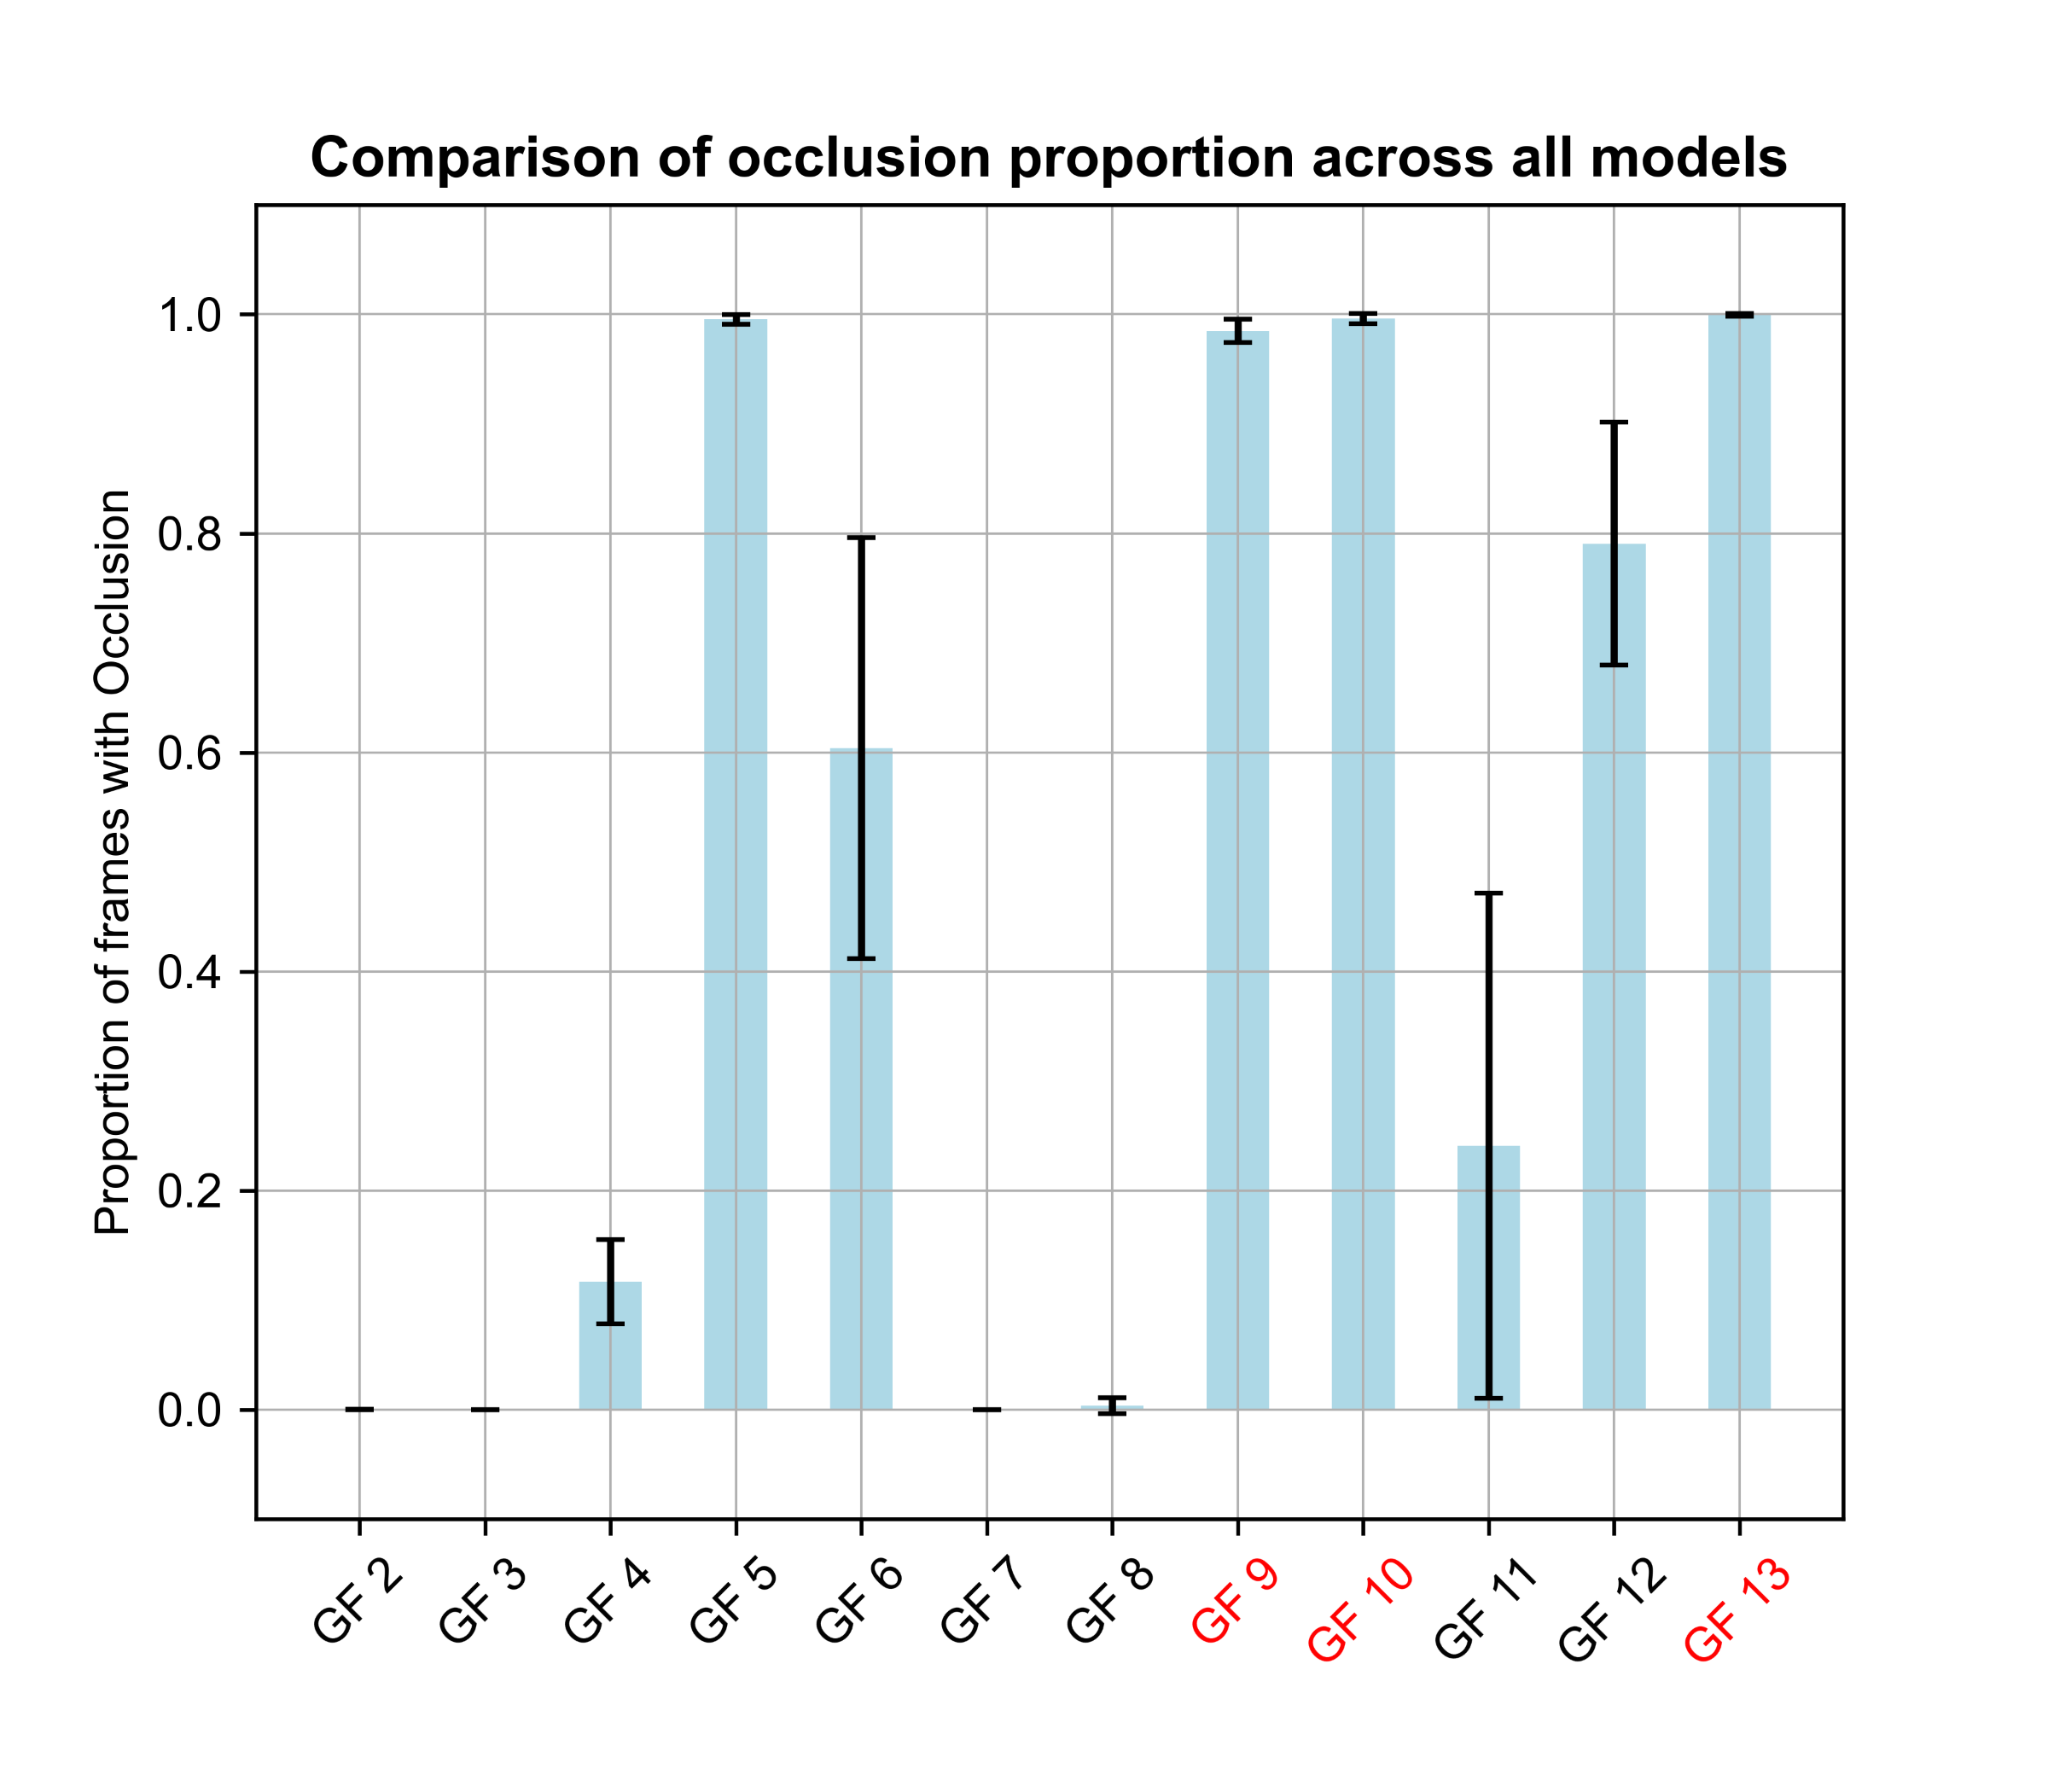
\includegraphics[width=0.50\textwidth]{Figures/occlusion_proportion_averaged.png}
\caption{Average occlusion analysis distinguishes glycoforms with low, medium, and high occlusion proportion. All five models for each glycoform were averaged for occlusion proportions, and are plotted with standard deviation represented in black bars. Axis labels in red indicate glycoforms with experimental dimerization data.}
\label{occlusion_results}
\end{figure}

% Talk about independence of model
To assess the dependence of these results on the starting structural model, for each glycoform we averaged the proportion of frames with occlusion across the five models and compared the means and associated standard deviations (Figure \ref{occlusion_results}). Occlusion proportions are consistent across the models for almost all the glycoforms, particularly those in the low and high occlusion batches. There is considerable variability in the glycoforms of the medium occlusion batch (GF 6, GF 11) but considering the consistency in the other models, this might result more from initial glycoform minimization/optimization than the model itself.

% Final thoughts about the occlusion
These results suggest that the dimer occlusion metric is independent of the initial model of human insulin. Since we cannot include a wild type in this analysis, there is no negative control for each glycoform set nor is there a way to predict percentage dimerization relative to wild type. But despite those drawbacks, this metric allows us to statistically differentiate results between glycoforms and the results are consistent with experimental data, and supports our hypothesis. The glycan-dimer occlusion metric, therefore, might be a useful predictor of dimerization propensity. Interestingly, the occlusion data suggests a unifying theme in glycan placement which might preclude dimerization: glycans that are large and those that are attached close to the dimer interface, especially residues ThrB27 and ThrB30.

\section{Conclusions}
The primary goal of our study is to develop metrics for screening the proteolytic stability and dimerization propensity of insulin based on MD simulations of monomers and their glycosylated analogs. The use of monomer simulations obviates the need of performing advanced sampling of more complicated systems, such as a protease-substrate complex or an insulin dimer. We also evaluated whether these metrics were independent of the initial configuration used. 

We examined four metrics based on two overarching hypotheses for proteolytic stability. The first is that the glycan could sterically hinder the scissile bonds or part of the binding sites, especially the P1 site, to prevent proteolysis, while the second is that the existence of the glycan disfavors configurations required for proteolytic degradation. From the first hypothesis, we derived two metrics, the SASA of the scissile bonds and the P1 sites. Both metrics were found partly predictive for assessing the proteolytic stability. Based on the second hypothesis, we examined $\beta$-sheet propensity of the P1--P3 region and the existence of glycan-involved hydrogen bonds that compete with the hydrogen-bonding network present in $\alpha$-chymotrypsin binding. The $\beta$-sheet propensity generally was not well correlated with proteolytic stability. The only residue whose $\beta$-sheet propensity suggested moderate predictiveness had excessively large error bars, making the metric less useful. Notably, the involvement of only a few atoms in the calculation naturally makes these 3 metrics relatively uncertain and less valuable. While the first 3 metrics are somewhat predictive or not predictive, long-lasting, stable glycan-involved hydrogen bonds, especially the ones involving residues PheB24 and ThrB27, were highly predictive in enhancing the proteolytic stability and independent initial wild-type model.  In particular, using glycosylation site ThrB27 is more likely to form hydrogen bonds with ThrB27 and PheB24 due to spatial proximity.

To assess dimerization propensity, we examined glycan occlusion of the dimer interface. This metric was consistent with the limited experimental data for dimerization and is free from starting model bias. There is no ability to include a wild-type model for comparison, which is a drawback of this metric. However, this metric showed clear, statistical differences between glycoforms with and without occlusion which translates to predictive differences in dimerization potential and is independent of starting model. Additionally, this metric suggests a generalizable glycosylation scheme that might preclude dimerization: large glycans and those attached near the dimerization interface (ThrB27, ThrB30). 

The presence of relatively little experimental data (13 proteolytic stability data points, 3 dimerization data points) means that it is difficult to make firm statistical conclusions about these screening metrics.  It is, however, the difficulty in generating experimental data that motivates the development of computational screening techniques.  Our framework presented here is widely applicable and allows easy screening of large numbers of insulin glycoforms. To further validate this approach, we will in the future apply this framework in a blind challenge to more complicated insulin glycoforms that are under experimental investigation. The results presented in this paper suggest that we are likely to be able to differentiate the structures with high proteolytic stability and low dimerization propensity from others, as long as the configurational ensembles of the investigated structures are sufficiently sampled. Building more complicated statistical learning models at the present time, such as decisions trees or multiple linear predictors is likely not viable, as the relative paucity of experimental data would cause high uncertainty of these weights and decision cuts. However, clearer metrics could possibly be identified in more sophisticated machine-learning approaches that essentially combine 3D coordinates of the systems of interest in a non-linear fashion. For example, recent deep learning frameworks~\cite{ward2021deep} like DiffNets appear capable of identifying subtle structural signatures that predict biophysical properties in future studies.


% % %===============================
% % % Acknowledgements and Funding
% % %===============================

\section{Data Availability}
As discussed in Section \ref{analysis_method}, most values reported in our results are averaged over different wild-type crystal structure models. For individual analysis result of each insulin glycoform, please refer to our \href{https://github.com/shirtsgroup/Glycoinsulin_project}{GitHub repository} of the project. The repository also contains input configurations/MD parameters and Python codes for data analysis. The outputs of the MD trajectories are too large to release as they are several terabytes in size and statistically representative outputs can be generated from the input files.   
\section{Acknowledgements}
Research reported in this publication was primarily supported by the National Institute of Biomedical Imaging and Bioengineering of the National Institutes of Health under award number R01EB025892. This work was also supported in part by the NIH/CU Molecular Biophysics Graduate Traineeship T32 GM065103 and the CAMS Innovation Fund for Medical Sciences (CIFMS 2021-1-I2M-026). The content is solely the responsibility of the authors and does not necessarily represent the official views of the National Institutes of Health.

%===============================
% Contributions
%===============================
\section{Author and Contributions}
Contributions based on CRediT taxonomy:

\noindent W.-T.H.: Conceptualization, Writing – Original Draft, Writing – Review \& Editing, Methodology, Investigation \\
D.A.R.: Writing – Original Draft, Writing -Review \& Editing, Methodology, Investigation  \\
T.S.: Conceptualization, Writing – Review \& Editing, Funding Acquisition \\
Z.T.: Conceptualization, Writing – Review \& Editing, Funding Acquisition \\
M.R.S.: Conceptualization, Writing – Review \& Editing, Supervision, Funding Acquisition \\

%===============================
% Disclosures
%===============================
\section{Disclosures}
MRS is an Open Science Fellow at and consults for Roivant Sciences.

%===============================
% Citations
%===============================
\bibliography{references}

%===============================
% The tables
%===============================
\clearpage

%===============================
% Figures
%===============================
\clearpage

\end{document}
